\documentclass[a4paper,twoside,11pt]{book}

\usepackage{epsfig}
\usepackage{epigraph}
\setlength\epigraphwidth{10cm}
\setlength\epigraphrule{0pt}

\usepackage{graphicx}
\usepackage{algorithm}
\usepackage{algorithmic}
\usepackage{verbatim}
\usepackage{multirow}
\usepackage[table]{xcolor}
\usepackage{color,colortbl}
\usepackage{url}
\usepackage{array}
\usepackage[bookmarks=true, pdftitle={
Algoritmos evolutivos en sincronización de semáforos en el Corredor de Garzón 	
	}, pdfauthor={Alvaro Acuña, Efraín Arreche}, colorlinks=true, linkcolor=black, citecolor=black, urlcolor=black]{hyperref}
\usepackage{bookmark}
\usepackage[spanish]{babel}
\usepackage[utf8]{inputenc}

\usepackage{amssymb}
\usepackage{amsmath}
\usepackage{amsthm}

\usepackage{ifthen}
\usepackage{fancyhdr}
\usepackage{setspace}
\usepackage[section]{placeins}
\usepackage[round,sort&compress]{natbib}



\usepackage{caption}
\usepackage{subcaption}
\usepackage{rotating}
\usepackage{xfrac}

\usepackage{appendix}
\usepackage{bibentry}


\theoremstyle{definition}
\newtheorem{mydef}{Definition}


\pagestyle{fancy}


\voffset = -1in
\topmargin = 30pt
\textheight = 650pt
\textwidth = 420pt
\headwidth = 450pt
\oddsidemargin = 0pt
\evensidemargin = 0pt


\renewcommand{\chaptermark}[1]{\markboth{#1}{}}
\renewcommand{\sectionmark}[1]%
	{\markright{\thesection\ #1}}
\lhead[\fancyplain{}{\bfseries\thepage}]%
	{\fancyplain{}{\bfseries\rightmark}}
\rhead[\fancyplain{}{\bfseries\leftmark}]%
	{\fancyplain{}{\bfseries\thepage}}
\cfoot{}
\makeatletter
\def\cleardoublepage{\clearpage\if@twoside \ifodd\c@page\else%
    \hbox{}%
    \thispagestyle{empty}%              % Empty header styles
    \newpage%
    \if@twocolumn\hbox{}\newpage\fi\fi\fi}

% algoritmos
\renewcommand{\ALG@name}{Algoritmo}
\renewcommand{\listalgorithmname}{Índice de \ALG@name s}

\makeatother

\hyphenation{}

\begin{document}

% tells bibentry to (re)use the bibliographic data from the standard BibTeX setup
\nobibliography*

% -- title page --
\pagenumbering{roman}
\begin{titlepage}
  \thispagestyle{empty}
  %\addtolength{\oddsidemargin}{0.5cm}
  \begin{center}
    ~\\[2.2cm]



    \textsc{\Huge Universidad de la República } \\[2.5cm]
    \textsc{\Huge PROYECTO DE GRADO } \\[0.5cm]
    \textsc{\Huge Ingeniería en Computación } \\[2.5cm]    
    \textbf{\Huge Algoritmos Evolutivos en } \\[0.2cm]
    \textbf{\Huge sincronización de semáforos en el } \\[0.3cm]
    \textbf{\Huge Corredor de Garzón } \\[1.5cm]    
    
    {\huge Alvaro Acuña} \\[0.2cm]
    {\huge Efraín Arreche} \\[0.2cm]
    {\Large 2014} \\[2.0cm]
    {\Large Supervisor: Sergio Nesmachnow} \\[1.0cm]

    \textsc{\large Centro de Cálculo - Instituto de Computación} \\[0.2cm]
    \textsc{\large Montevideo, Uruguay} \\[1.5cm]

  \end{center}
  \vfill
\end{titlepage}
{
  \thispagestyle{empty}
  %\addtolength{\evensidemargin}{-1.5cm}
  ~\\[16cm]
  Algoritmos Evolutivos en sincronización de semáforos en el Corredor de Garzón \\[0.05cm]
  Acuña, Alvaro - Arreche, Efraín \\[0.05cm]
  Proyecto de Grado \\[0.05cm]
  Instituto de Computación - Facultad de Ingeniería \\[0.05cm]
  Universidad de la República \\[0.05cm]
  Montevideo, Uruguay, Marzo de 2015 \\[0.05cm]
  \vfill
  \cleardoublepage
}
\setcounter{page}{1}
\cleardoublepage

{
\thispagestyle{empty}
~\\[0.2cm]
\begin{center}
    \textsc{\huge Algoritmos evolutivos en  } \\[0.2cm] 
    \textsc{\huge sincronización de semáforos en el  } \\[0.2cm]         
    \textsc{\huge Corredor Garzón} \\[1cm]
    \textsc{\Large Resumen}
\end{center}
~\\[0.2cm]
\textbf{\large 
El proyecto propone el estudio de la sincronización de semáforos como problema de optimización multiobjetivo, y el diseño e implementación de un algoritmo evolutivo para resolverlo con alta eficacia numérica y desempeño computacional. \newline \newline
Se toma como aplicación la sincronización de semáforos en el Corredor Garzón  (Montevideo, Uruguay). La cantidad de cruces, calles, tráfico y semáforos lo hace un problema interesante desde el punto de vista de su complejidad. Además se ha admitido, por parte de las autoridades responsables, los problemas relacionados con la sincronización de los semáforos, por lo que todavía hay espacio para la mejora de los tiempos promedio de los viajes.  \newline \newline
El problema de sincronización de semáforos es NP-difícil y no existe (hasta el momento) un método determinístico que lo resuelva. Se buscará mediante un algoritmo evolutivo llegar a una configuración aceptable de los semáforos maximizando la velocidad media tanto de ómnibus como de otros vehículos.
El enfoque seguido es la obtención de datos reales relacionados a la red vial, tráfico y configuración de semáforos y la utilización del simulador de tráfico SUMO para generar los datos requeridos por el algoritmo.
\newline \newline
El análisis experimental consiste en comparar los resultados del algoritmo con los valores obtenidos en la simulación de la realidad actual y además crear un escenario alternativo con modificaciones con el objetivo de obtener mejores métricas. Los resultados muestran que el algoritmo logra una mejora de hasta  24.2 \% (21.40 \% en promedio) en el valor de fitness comparando con la realidad actual, mientras el escenario alternativo obtiene una mejora de hasta 37.1 \% (34.7\% en promedio) en el valor de fitness.
 } 	
	~\\[1.0cm]
    \textbf{\large Palabras clave: Optimización, Sincronizacion semáforos, Corredor Garzón, simulación de tráfico,  Algoritmo Genetico multiobjetivo y paralelo,  escenario real, Cluster}

}
\cleardoublepage

\cleardoublepage

% -- table of contents --
%
%\setcounter{tocdepth}{4}
\tableofcontents
\listoffigures
\listoftables
\listofalgorithms
\cleardoublepage


\cleardoublepage

% --- Main Document --- --- --- --- --- --- ---
%
\mainmatter
\setcounter{page}{1}
\pagenumbering{arabic}
%

\chapter{Introducción}
\epigraph{ \textit{He llamado a este principio, por el cual cada pequeña variación, si útil, es preservada, con el término de Selección Natural}}{--- Charles Darwin, El origen de las especies}

En esta sección se pretende introducir al lector en el contexto general donde se desarrolla este trabajo así como los objetivos buscados.

\section{Motivación y contexto}

Los algoritmos evolutivos han demostrado su utilidad en problemas complejos y particularmente uno de ellos es la sincronización de semáforos. Se busca desarrollar un algoritmo que logre resolver este problema con buenas métricas.
Por la flexibilidad inherente de este algoritmo es que no está destinado a resolver el problema en una zona en particular sino que se podría aplicar en forma general.

En este sentido se eligió la zona del corredor Garzón que presenta particularidades que la destacan y la hacen interesante desde el punto de vista de la investigación. Su complejidad viene dado por el largo del tramo, la cantidad de cruces, la complejidad y cantidad de semáforos en cada uno de ellos, las distintas reglas de tráfico aplicadas a cada tramo como por ejemplo exclusividad del ómnibus, o distinción para doblar a la izquierda, tráfico vehicular y transporte publico, calles no paralelas, entre otros.

Por tanto al comprobar que el algoritmo obtiene un buen rendimiento en esta situación se puede tener confianza de que se comportaría adecuadamente en otras zonas que no presentan tanta complejidad.



\newpage

\section{Objetivos}

Estos son los objetivos básicos que se plantearon al inicio del  proyecto.

\begin{itemize}
	\item Estudio del problema del tráfico y la sincronización de semáforos.
	\item Revelamiento de información sobre trabajos relacionados en este ámbito.
	\item Creación de un algoritmo evolutivo paralelo que resuelva el problema en la zona del corredor Garzón.
	\item Creación de un mapa y  configuración relativa a semáforos, tráfico y reglas de tránsito que sea precisa y obtenida de la realidad actual.	
	\item Aplicar técnicas de computación de alto desempeño para aumentar el rendimiento de la solución.

\end{itemize}

 
\section{Enfoque}

Desde un primero momento se intento dotar al proyecto de una buena aproximación de la realidad, en tal sentido se realizaron reuniones con el Ing. Juan Pablo Berta del Servicio de Ingeniería de Tránsito de la Intendencia de Montevideo en Agosto del  2014 y con el Ing. Daniel Muniz del departamento de Informática de la Intendencia en Setiembre de 2014 para conocer la situación del tráfico capitalino, aprender de su experiencia y obtener datos que nos fueran útiles para el proyecto.


Buscando una aproximación aun más precisa se realizaron trabajos de campo para determinar la configuración de los semáforos, la densidad de tráfico y el tiempo de recorrida. El mapa y la frecuencia de ómnibus son de acceso publico así como el simulador utilizado.

Se creará un programa que implemente un algoritmo evolutivo multiobjetivo que utiliza un simulador de tráfico para obtener las métricas a optimizar. Se busca obtener una nueva configuración de semáforos que en las simulaciones se comporte mejor que la situación actual basándonos en la velocidad promedio de ómnibus y del resto de los vehículos.

Dada la complejidad del problema el algoritmo será paralelo y se utilizara la plataforma Cluster fing para poder acelerar el tiempo real de procesamiento. Además se realizará un escenario alternativo con modificaciones de la realidad actual con el objetivo de mejorar las métricas.

\section{Limitaciones y alcance}

La zona modelada comprende todo el tramo de el Corredor Garzón y dos caminos paralelos a ambos lados, que dada la configuración de las calles las cuales corren en diagonal fue un proceso complejo.
El revelamiento de tráfico hecho in-situ fue realizado para un número determinado de calles que contiene a Garzón y cinco cruces representativos. Se busca una aproximación útil y no un estudio detallado sobre el tráfico en la zona.

Como lo que se pretende modelar es el tráfico vehicular y transporte publico no se realiza una simulación de peatones.


\section{Aportes}

\begin{itemize}
	\item Se desarrollo un sitio web en la siguiente direccion: \url{http://www.fing.edu.uy/inco/grupos/cecal/hpc/AECG} donde los interesados podrán acceder para encontrar información sobre el proyecto y los resultados. 
	\item Se realizó un \emph{paper} en idioma ingles de 10 paginas con el objetivo de presentarlo en conferencias internacionales.
	\item El proyecto fue presentado en Ingeniera demuestra 2014, siendo bien recibido por el publico. Constatando de primera mano que la problemática es real y llegando a la conclusión que los Ingenieros tienen las herramientas necesarias para solucionar problemas que afectan directamente a la sociedad.

\end{itemize}






\section{Estructura del documento}
En el siguiente capitulo se hace un repaso sobre fundamentos teóricos necesarios para comprender el resto del trabajo. Se da información sobre corredores y en concreto el Corredor Garzón, así como un repaso breve sobre algoritmos evolutivos y simuladores de tráfico. Además se muestran los trabajo relacionados enfocando en algoritmos genéticos para la sincronización de semáforos.

En el capítulo 3 se explica como se modela el problema y la arquitectura diseñada  para resolverlo. Luego se comenta el trabajo de campo realizado para obtener datos de la realidad utilizados en la solución. Además se detalla el algoritmo genético utilizado así como la biblioteca y herramientas usadas.

El capítulo 4 cuenta con la descripción de los escenarios, los resultados de la evaluación del algoritmo y las comparaciones realizadas. En este caso tenemos el escenario que representa la situación actual y también un escenario alternativo con modificaciones los cuales se evalúan con el algoritmo. Además se realizan pruebas para comprender como varia el algoritmo al modificar su función de fitness y se realiza un breve análisis de la eficiencia computacional del algoritmo.

El capítulo 5 da las conclusiones finales y el trabajo a futuro que se puede realizar.







\chapter{Marco Teórico}
Este capítulo aborda el marco teórico necesario para comprender el desarrollo de los capítulos posteriores. Se analiza el problema del tráfico en general y las soluciones propuestas para manejarlo incluyendo la construcción de corredores exclusivos para el transporte público. En este contexto se presenta la descripción del Corredor de Garzón y sus problemas. Luego se presenta un relevamiento sobre simuladores de tráfico y la teoría detrás de los algoritmos evolutivos. Para finalizar, se incluye un relevamiento de trabajos relacionados para mostrar y comentar otras variantes del problema y soluciones propuestas en la literatura del área.
\section{Problema del tránsito vehicular}

En gran parte del mundo se está produciendo un crecimiento sostenido del parque automotor, lo cual ocasiona una serie de problemas relacionados con el agravamiento de las congestiones vehiculares que afectan la calidad de vida de las personas \citep{Cepal2003}. Este problema tiene un gran impacto en el desarrollo de las ciudades, por lo que es un componente principal en los planes estratégicos para su crecimiento.

La congestión ocasiona una progresiva merma de la velocidad promedio de circulación, con la consecuencia del incremento en la duración de los viajes y del consumo de combustible. Esto repercute en la contaminación atmosférica y sonora que impacta directamente en la salud de las personas; además, se genera una exigencia en las vías de tránsito que ocasiona un deterioro mayor de calles y rutas.

Uruguay y en particular Montevideo, no escapa a este fenómeno. El aumento del parque automotor en la capital del país está en ascenso constante desde el 2005 \citep{INE2014}, y según proyecciones el crecimiento seguiría en un promedio de 4.5\% anual hasta el 2020 \citep{BBVA2013}. Este crecimiento viene de la mano con el sostenido aumento de las ventas de vehículos desde el 2003 como se aprecia en la Figura \ref{fig:ventas_autos}.

Los expertos indican que la situación de congestión ya está instalada en la ciudad y la infraestructura vial no acompasó este crecimiento. Montevideo es la ciudad con más semáforos por automóvil en Latinoamérica, con más de 620 cruces semaforizados, alguno de los cuales no están coordinados \citep{Subrayado2013}.

\begin{figure}[H]
	\centering
	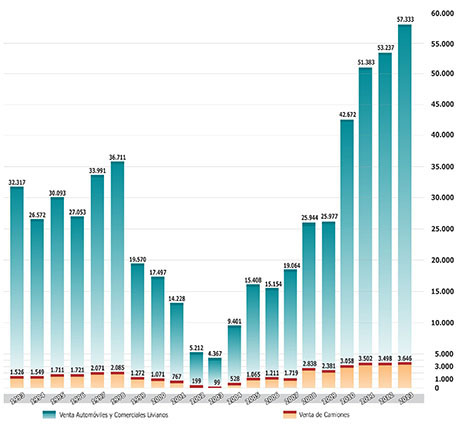
\includegraphics[width=0.9\linewidth]{Figures/ventas_autos}
	\caption[Evolución de la venta de automóviles en Uruguay]{Evolución de la venta de automóviles por año. El valor más bajo corresponde al año 2003, y el más alto 2013. Imagen extraída de {http://www.autoanuario.com.uy} .	
	}
	\label{fig:ventas_autos}
\end{figure}

En un contexto global, el crecimiento en la circulación de automóviles provoca que baje el nivel de aceptación del transporte público, cuyo servicio en general es ineficiente. Para resolver este problema las autoridades suelen optar por instrumentar sistemas de transporte costosos como los \emph{metros}, pero se ha demostrado que existen otras opciones viables como el BRT (Bus Rapid Transit / ómnibus de tránsito rápido)\citep{BRT_Dial}.

En el caso de la ciudad de Montevideo, para solucionar este problema se está implementando el Plan de Movilidad Urbana \citep{PlanMovilidad} con el objetivo de mejorar la eficiencia del transporte público y democratizar el acceso al mismo. El sistema de transporte está inspirado en un BRT con la construcción de varios corredores exclusivos en la ciudad. En la siguiente sección se presenta más información sobre los BRT, corredores urbanos y en particular el Corredor de Garzón.

\section{Corredores urbanos de tráfico}
El corredor urbano de tráfico, también llamado \emph{corredor segregado}, se caracteriza por una separación física entre el carril de circulación de los ómnibus y los carriles para el resto del tráfico. 
Esta es la principal diferencia con un concepto similar llamado \emph{carril de sólo bus}, en donde se separan los carriles por líneas horizontales pintadas en la calle indicando que sólo pueden circular ómnibus. Los carriles de \emph{sólo bus} suelen ser poco exitosos como medida de agilizar el tráfico de transporte colectivo por falta de control que evite que el tráfico los invada. 

En el caso de Montevideo el carril \emph{sólo bus} está sobre la derecha, por lo que los vehículos privados lo invaden al virar a la derecha y los taxis lo necesitan invadir para levantar/dejar pasajeros. Al ubicar los corredores alineados en el medio de las vías de tráfico, se evitan esos problemas.  

Las ciudades de países en vías de desarrollo deben estudiar si pueden instalar corredores, su objetivo fundamental es para conseguir mayores velocidades en el sistema. Existen muchas posibilidades de implementación y no todas pueden ser aplicables por el contexto zonal, cultural o de inversión necesaria.

\begin{figure}[H]
	\centering
	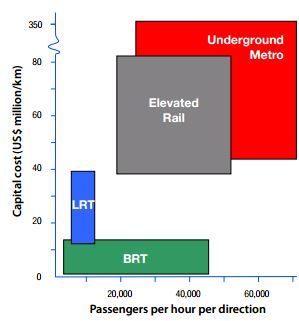
\includegraphics[width=0.9\linewidth]{Figures/costo_transporte}
	\caption[Gráfica de costos de transporte en función de la gente transportada.]{Gráfica de costos de transporte en función de la gente transportada.- Imagen original extraída de \citep{ITDP}		
	}
	\label{fig:Grafica de costos de otros medios de transporte}
\end{figure}

BRT es una solución innovadora, de alta capacidad y de menor costo para el transporte público que puede alcanzar el rendimiento y los beneficios de sistemas ferroviarios, con un costo significativamente menor. Se trata de un sistema integrado de movilidad basado en ómnibus para el transporte de los pasajeros a sus destinos de manera rápida y eficiente. Al mismo tiempo, ofrece la flexibilidad necesaria para satisfacer una variedad de condiciones locales. Los elementos del sistema de BRT pueden ser fácilmente personalizados a las necesidades de la comunidad e incorporan tecnologías de última generación de bajo costo que atraen a más pasajeros y en última instancia ayudan a reducir la congestión de tráfico en general.

Un BRT contiene características similares al tren ligero o al sistema de metro, por lo que es mucho más confiable, conveniente y más rápido que los servicios regulares de ómnibus. Entre sus características principales se destacan el uso de carriles exclusivos para el ómnibus, con un alineamiento central del carril y un largo mínimo de 3 km. El uso de ómnibus de gran capacidad para transportar un número mayor de personas, la compra de pasajes fuera del ómnibus, que agiliza la entrada de pasajeros y que el ómnibus tenga prioridad sobre otros vehículos en las intersecciones. Con las especificaciones adecuadas, un BRT es capaz de evitar las causas de los retrasos que suelen tener los servicios regulares de ómnibus, como estar atrapado en el tráfico y hacer cola para pagar a bordo. 

Para crear una definición común de BRT y calificar los sistemas existentes alrededor del mundo,  evaluando su funcionamiento basado en las mejores practicas internacionales existe el standard BRT creado por \citet{brt_standar}. Su principal objetivo es brindar una mejor experiencia a los pasajeros, con un costo económico acorde e impacto ambiental positivo. El standard cuenta con un método para calcular el puntaje del corredor y determinar su nivel de calidad. 

En la siguiente sección se presenta un análisis exhaustivo de varios puntos presentados en el standard BRT en relación con el caso de estudio del proyecto: el Corredor Garzón.

	
\section{Corredor Garzón}	


El Corredor Garzón fue construido como parte del Plan de Movilidad Urbana que incluye otros corredores en la ciudad de Montevideo. \citep{PlanMovilidad}. El corredor conecta los barrios de Colón, Sayago, Belvedere y Paso Molino. Tiene una extensión de 6.5km con 24 cruces semaforizados, en donde se encuentran calles importantes como Millán, que conecta con una autopista (Ruta 5), y Bulevar Batlle y Ordoñez, la cual tiene una gran densidad de tráfico. Es importante aclarar que el corredor Garzón no es sólo una conexión de extremo a extremo, ya que se encuentra en una zona densamente poblada cuyos barrios tienen al corredor como la principal vía de movilidad.

\begin{figure}[H]
	\centering
	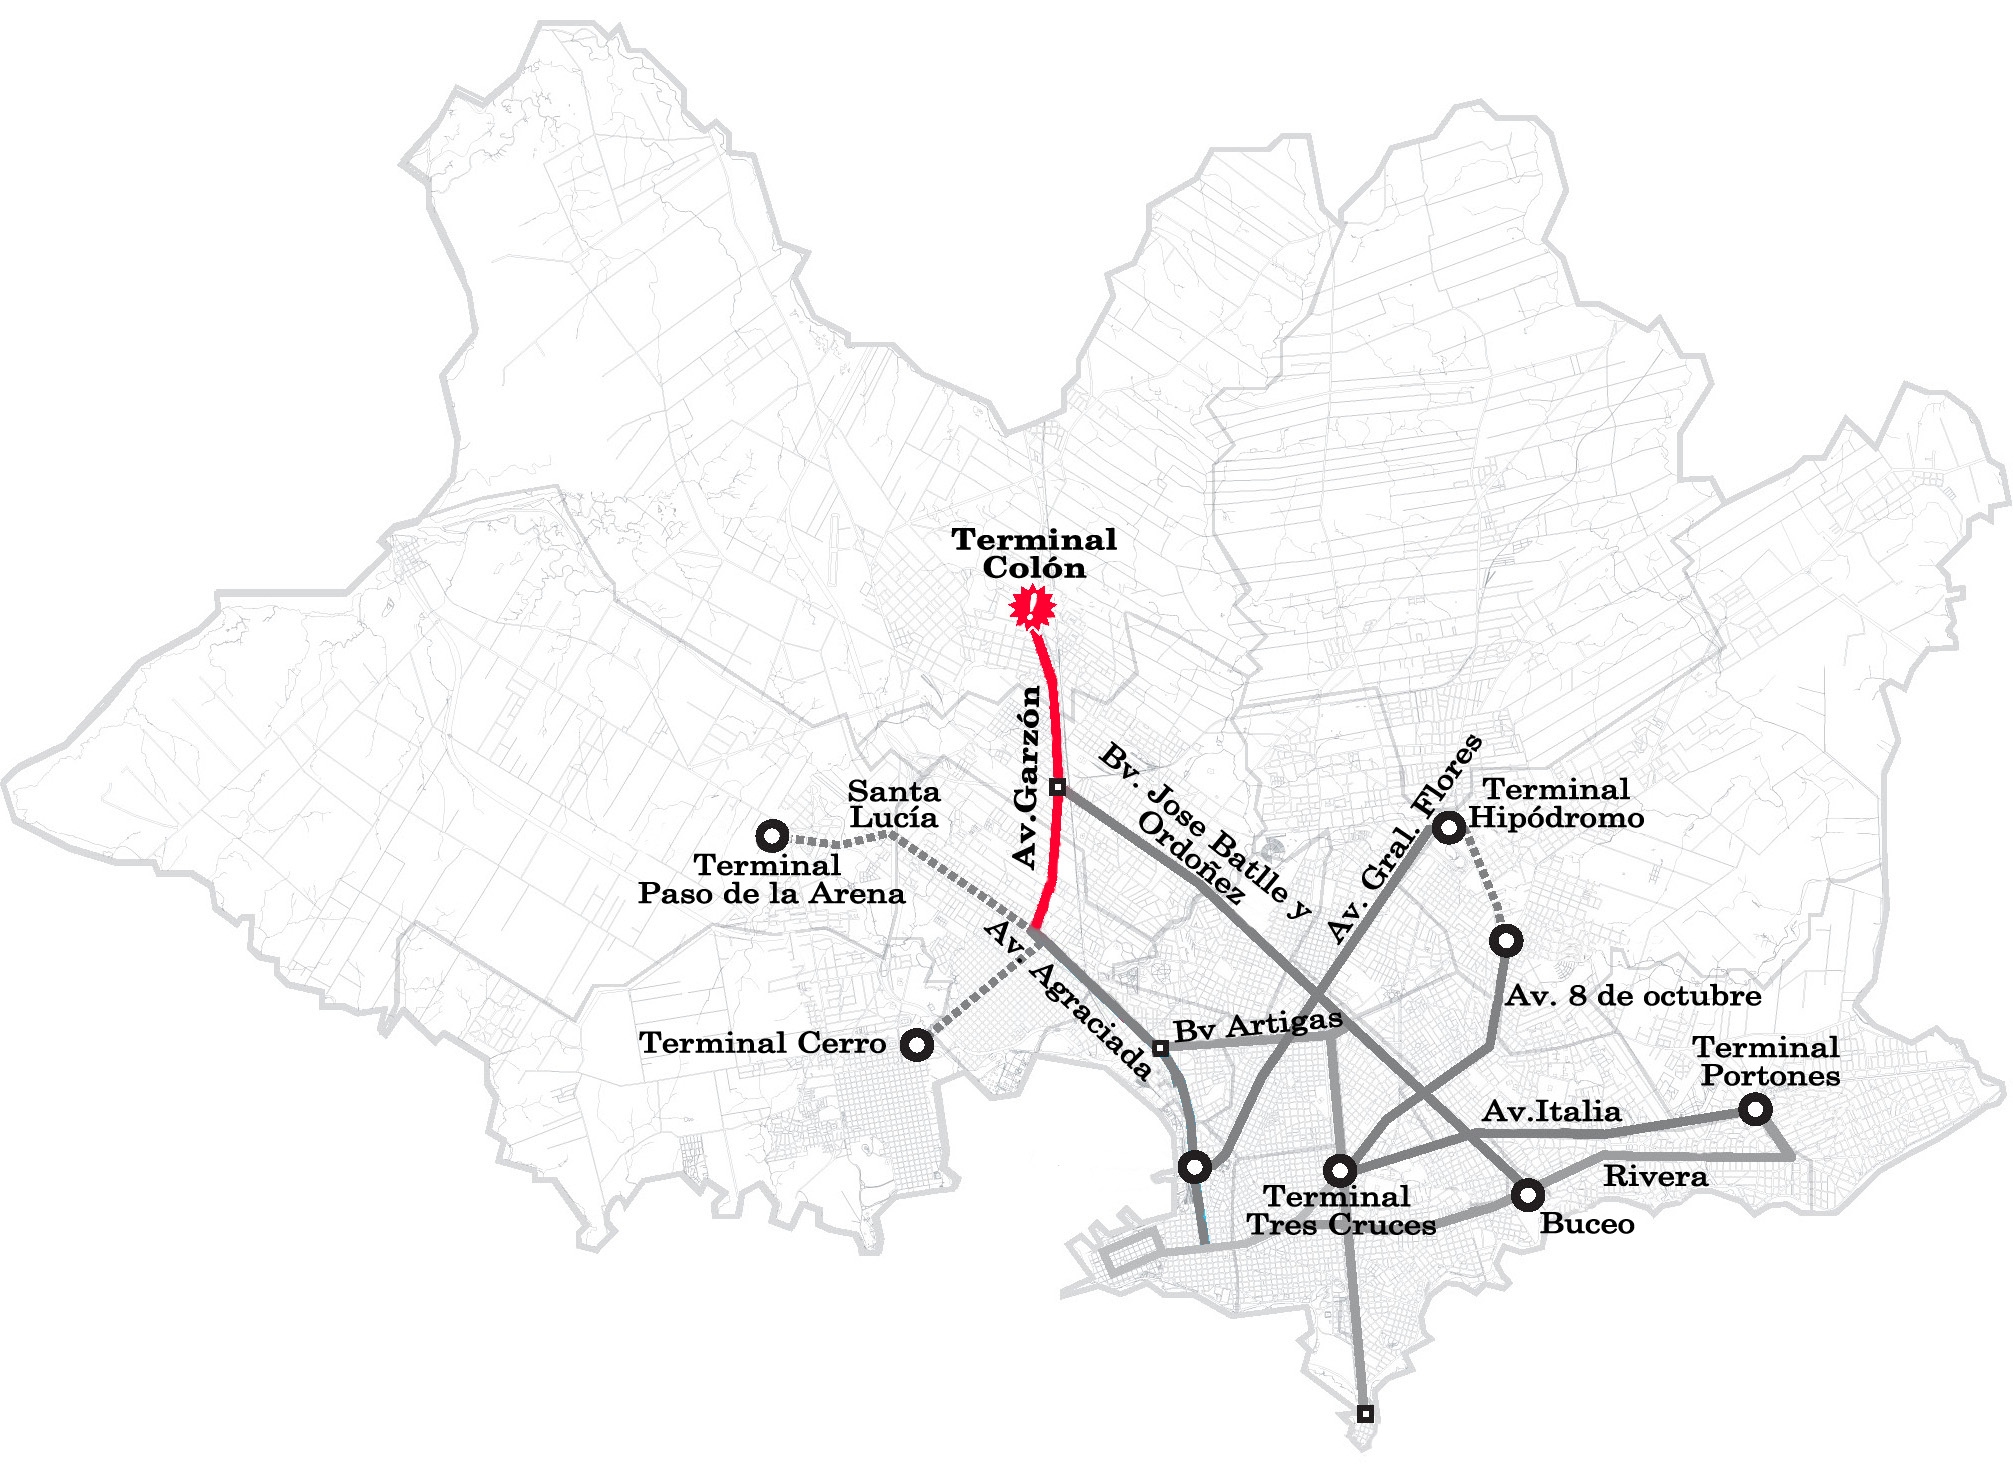
\includegraphics[width=0.99\linewidth]{Figures/Mapa_Garzon_0}
	\caption[Localización del Corredor de Garzón en Montevideo]{Localización del Corredor de Garzón en Montevideo, referenciado en color rojo - Imagen original extraída de www.montevideo.gub.uy		
	}
	\label{fig:Grafica de costos de otros medios de transporte}
\end{figure}

Como se aprecia en la Figura \ref{fig:perfil_garzon}, el corredor consiste básicamente de tres calles paralelas e independientes. Dos calles cuentan con dos carriles de una sola mano y entre medio de éstas se encuentra una calle de doble vía con un carril para cada vía, que es exclusivamente usado por ómnibus urbanos durante el día y por ómnibus urbanos y suburbanos en la noche.

Basándose en el standard antes mencionado, el Corredor de Garzón cumple con la definición de BRT por las siguientes características:
\begin{itemize}
	\item Largo mínimo del corredor: 3 km de corredor exclusivo.
	\item Vía de ómnibus dedicada: al tener un 90\% de segregación física dentro del corredor.
	\item Alineación de la vía del ómnibus: por estar constituido por dos carriles centrales para el ómnibus en medio de los carriles de otros vehículos.
	\item Tratamiento de intersecciones: por prohibir algunos virajes a la izquierda y el carril de ómnibus tener prioridad en la mayoría de las intersecciones.
\end{itemize}


Analizando los puntos presentados en el standard como recomendaciones para la implementación de corredores urbanos, hay algunas características que no están totalmente aplicadas al Corredor Garzón, entre las que se destacan:

\begin{itemize}
	\item Cobrar el boleto fuera del ómnibus: uno de los factores más importantes para mejorar la experiencia del usuario, así como también la velocidad en zonas de mucha carga, es que existan al menos algunas estaciones (no solo paradas de ómnibus) donde el boleto se cobre (o se use tarjeta de transporte) al entrar a la estación.
	\item Servicios expresos o limitados: Una forma de mejorar las velocidades de operación consiste en crear líneas que no se detengan en todas las paradas (evitando aquellas paradas con menor demanda de pasajeros) y poner más ómnibus en la calle.
	\item Carril extra para adelantarse en paradas: este carril resulta crítico en sistemas de transporte colectivo de gran porte para poder manejar los servicios expresos. En sistemas de baja demanda es una buena inversión y en el caso del corredor de Garzón podría permitir que los servicios suburbanos funcionaran durante todo el día por el corredor, mejorando así el transporte público y privado.
	\item Distancia entre paradas e intersecciones: según el standard, la mínima distancia entre la intersección y la parada es de 26 m, pero idealmente deberían ser 40 m para evitar retrasos. En el Corredor Garzón las paradas están sobre las intersecciones y hay varias paradas donde se detiene más de una línea de ómnibus. Esto puede ocasionar problemas, dado que mientras uno o dos ómnibus ya realizaron la parada y esperan por el semáforo, los demás que lleguen generarán una fila aguardando por detenerse en la parada para levantar a los pasajeros y posiblemente luego, cuando lleguen al cruce, no tendrán la luz verde.
	\item Tener estaciones centrales o conexión entre paradas: la ausencia de paradas en el centro de los dos carriles de ómnibus hace que el diseño tenga una construcción más cara (hay que hacer dos paradas). El hecho de que no haya una conexión física por la cual el pasajero pueda cambiar de recorrido de un lado al otro sin tener que cruzar la calle, lo hace menos eficiente y más inseguro.
	\item Distancia entre estaciones:  las paradas deberían estar a una distancia de entre 300 m y 800 m, siendo 450 m la distancia óptima tanto para el pasajero como para el transporte.
	\item Puertas de los ómnibus: con el fin de mejorar el flujo y volumen de pasajeros, sería conveniente contar con dos puertas anchas o más de tres puertas comunes.
	\item Semáforos: un corredor debe de funcionar al igual que una autopista, en el sentido de que una vez que se entra debería ser posible mantener la velocidad máxima sin tener que detenerse con frecuencia, por lo que no deberían de haber semáforos cerca uno de otro. De haberlos, la sincronización será la clave para minimizar los tiempos de espera.
	\item Calles paralelas: tener calles paralelas es de vital importancia para un corredor, ya que una de las formas de minimizar los tiempos de espera es prohibir los giros a la izquierda, y una calle paralela provee la facilidad de poder realizarlo.
	\item Giro a la derecha con luz roja: actualmente, en muchos países se encuentra reglamentada una ley que permite a los conductores doblar a la derecha con luz roja, ya que la misma (a menos que se especifique) es tomada como un cartel de pare \emph{solamente} para doblar a la derecha. En donde esta aprobada esta ley acorta los tiempos de luz verde de las transversales, mejorando así la velocidad promedio en los corredores o calles importantes.
	\item Mejor calidad de estaciones: las paradas deberían ser a prueba del clima, con puertas corredizas que abren cuando hay un ómnibus (para que nadie caiga al corredor), con información al pasajero en tiempo real, etc. Estas especificaciones no harían al corredor más rápido pero si más seguro, cómodo y confiable.
\end{itemize}


\begin{figure}[H]
	\centering
	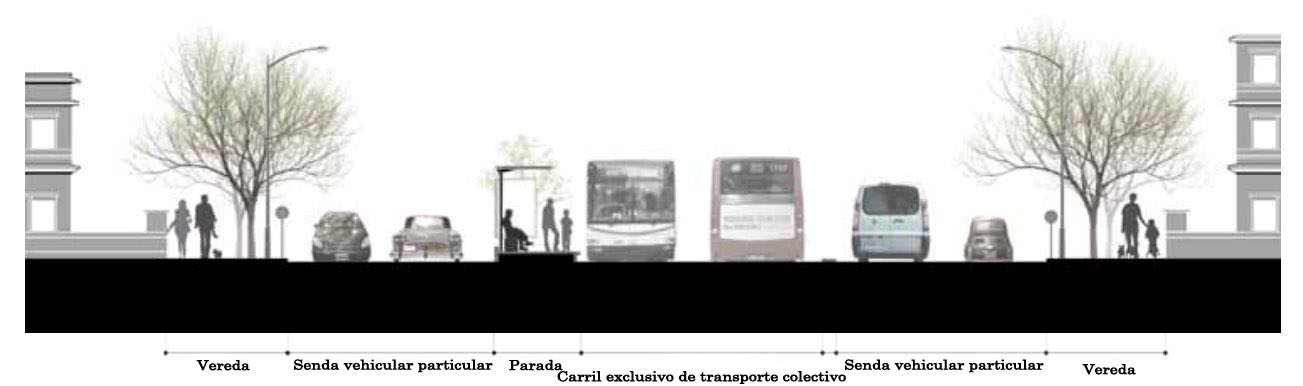
\includegraphics[width=0.9\linewidth]{Figures/busway_configuration}
	\caption[Perfil propuesto para el corredor Garzón.]{Perfil propuesto para el corredor Garzón desde San Quintín a Camino Colman - Imagen original extraída de \citep{PlanMovilidad}
	}
	\label{fig:perfil_garzon}
\end{figure}

Desde su construcción, el corredor ha recibido críticas debido a que su principal objetivo de agilizar el transporte público no fue cumplido. Luego de varios intentos de mejoras al respecto, se ha vuelto a una situación que implica la misma velocidad promedio para el transporte público que existía antes de realizar el corredor \citep{olivera2015}.

Las autoridades municipales admitieron que se han cometido errores en el diseño del corredor, y que no se ha logrado sincronizar los semáforos en las vías de tránsito que lo componen \citep{olivera2013}. Un buen funcionamiento de los semáforos es fundamental para asegurar que el tráfico circule con eficiencia y a la vez aporte seguridad a los peatones. A continuación se tratará específicamente el tema de sincronización de semáforos, que da la motivación para este proyecto. 


\section{Sincronización de semáforos}
Los métodos utilizados para la optimización del tráfico tienen como objetivo mejorar el flujo de vehículos en una red vial. Estos métodos se pueden clasificar en dos categorías: influir en el comportamiento de los conductores (mediante la configuración de semáforos, introducción de señalizaciones, etc) o realizar modificaciones en las vías de tráfico (agregar nuevos carriles, ensanchar calles, etc). Las modificaciones de infraestructuras pueden producir mejoras drásticas, pero requieren una inversión monetaria y un espacio físico que muchas veces no está disponible. Por esta razón, los métodos destinados a influir en el comportamiento de los conductores se presentan como una mejor opción o inclusive como única opción en muchos escenarios.

Los métodos para la sincronización de semáforos se encuentran entre los más efectivos para agilizar el tránsito y no generar congestiones. Estas técnicas permiten aumentar la velocidad promedio de los viajes y mejorar las perspectivas de desarrollo de la ciudad así como la calidad de vida de sus habitantes. 

Un concepto importante en el manejo de semáforos es el de \emph{fase}, que se refiere a una configuración especifica de luces de semáforos en una intersección de calles, que permiten el movimiento de ciertos flujos de tráfico. Como se ve en la Figura \ref{fig:fases} cada intersección puede tener diferente número de fases y también distintas duraciones. Las fases suelen ser configuradas y establecidas manualmente por técnicos especializados basados en su experiencia, aunque en ciertas ocasiones se utilizan simulaciones computacionales para obtener configuraciones apropiadas. 

\begin{figure}[H]
	\centering
	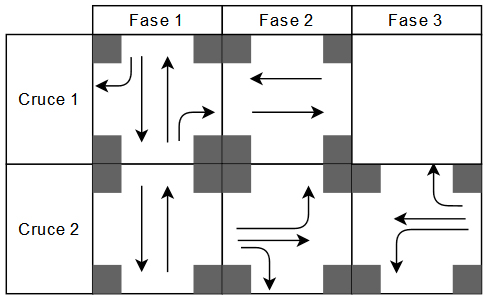
\includegraphics[width=0.8\linewidth]{Figures/fases1}
	\caption{Distintas fases de semáforos para dos cruces en una red de tránsito.}
	\label{fig:fases}
\end{figure}

Existen tres parámetros importantes a tener en cuenta que determinarán el comportamiento del sistema: la duración de fase, los ciclos de las luces y los valores de \emph{offset}. 
A continuación se explica cada uno de ellos:


\begin{itemize}
 	\item Duración de fase: Se refiere a la duración en que una configuración especifica de las luces de los semáforos esta activa en una intersección. Un conjunto de las luces estará en verde y otras en rojo, determinando qué vía esta habilitada para cruzar en ese momento. La elección correcta de este parámetro es fundamental; las calles con una densidad de tránsito mayor tendrían que tener más tiempo asignado para cruzar. Realizar la optimización individual de cada intersección no tiene por qué conducir a una solución óptima de toda la red vial, ya que puede ocasionar cambios en el flujo vehicular que afecte otras secciones de la red. Por esta razón es conveniente utilizar un enfoque global al modelar una solución.
 	
 	\item Duración del ciclo: Un ciclo representa un conjunto de fases. En general la duración de un ciclo es la suma de las duraciones de las fases. Como indica su nombre, el ciclo se repetirá una vez que se completa. La duración puede incrementarse o decrementarse para permitir mayor cantidad de repeticiones de las fases.
 	% Otro punto a considerar, sobre todo en intersecciones complejas, es el orden en el cual las fases son ejecutadas.
 	
 	\item \emph{Offset}: Indica en qué fase comienza el ciclo o en qué instante de tiempo, permitiendo que las intersecciones comiencen su ciclo en diferentes momentos. Este concepto es muy importante para sincronizar un flujo de tráfico en lo que se conoce como \emph{línea verde}, en donde los vehículos logran pasar todas las intersecciones sin detenerse.
\end{itemize}

Los parámetros mencionados anteriormente pueden ser utilizados a la hora de sincronizar los semáforos de una zona, buscando una optimización global de la red vial. También se debe tener en cuenta la implementación de soluciones seguras desde el punto de vista de las ordenanzas de tránsito, siendo lo más básico que no existan intersecciones donde los flujos vehiculares estén habilitados para cruzar al mismo tiempo.

Los métodos para lograr la coordinación necesaria entre semáforos incluyen van desde simples mecanismos de reloj a sistemas computarizados que se ajustan en tiempo real con la ayuda de sensores en la calle. Estos métodos pueden clasificarse como estrategias de tiempo fijo o de tiempo dinámico auto-ajustable.

Se considera al problema de sincronización de semáforos como un problema de optimización NP-difícil \citep{yang1996model}, por lo que los métodos de resolución exactos solo son útiles para resolver instancias de tamaño reducido. Por esta razón se suelen utilizar diferentes métodos heurísticos, alguno de los cuales se describen en la sección de trabajos relacionados. Entre los métodos más desarrollados y efectivos para resolver el problema están los algoritmos evolutivos, en particular los algoritmos genéticos, que serán explicados a continuación.

\section{Algoritmos Evolutivos}

Los algoritmos evolutivos (AE) son un conjunto de técnicas metaheurísticas para la resolución de problemas complejos que se inspiran en la evolución natural. Los AE trabajan sobre una población de individuos que representan una solución y utilizan mecanismos de selección, reproducción y técnicas para mantener la diversidad para calcular soluciones de buena calidad para el problema \citep{spears2000evolutionary}. 

Un AE se describe como una técnica iterativa que busca en cada paso mejorar las soluciones por medio de operadores de exploración y explotación, basado en un criterio predefinido a maximizar o minimizar.

Se pueden destacar cuatro etapas en la ejecución del AE:

\begin{itemize}
	\item Evaluación: Para cada individuo de la población se determina un valor de aptitud \emph{fitness} en relación a su capacidad para resolver el problema. 
	\item Selección: Proceso en donde se eligen cuales son los individuos que sobrevivirán a la siguiente generación y sobre los cuales se aplicarán los operadores evolutivos.
	\item Operadores evolutivos: Se aplican combinaciones entre individuos (cruzamiento), y modificaciones aleatorias de individuos(mutación). Los operadores generan nuevos individuos que sustituirán a los existentes en la población.
	\item Reemplazo: Se produce el recambio generacional, sustituyendo a la antigua población por una nueva que podría tener sobrevivientes de la anterior o solamente nuevos individuados generados en la etapa de aplicación de los operadores evolutivos.
\end{itemize}

Se han desarrollado enfoques de algoritmos de optimización que aplican estos conceptos, las más relevantes se describen a continuación:

\begin{itemize}

	\item Estrategias de Evolución: Propuesto por \citet{Ingo1971}, fue originalmente propuesto como un método de optimización utilizando individuos que codifican números reales en problemas relacionados al diseño de ingeniería. Su característica principal es que utilizan el operador de mutación como motor para la evolución. Sin embargo, modelos más recientes agregan otro tipo de operadores, incluyendo cruzamiento.
	\item Programación genética: Intenta generar un programa de computación para resolver una tarea específica, aplicando técnicas evolutivas. Cada individuo puede ser un programa que es representado en forma de árbol, donde cada nodo del árbol tiene una operación y los nodos terminales un operando, de esta manera se facilita la evaluación de expresiones matemáticas. La función de aptitud se refiere a que tan cerca de resolver la tarea se encuentra el individuo \citep{Koza1992}.
	\item Algoritmo Genético: Es considerado el mas popular de los AE, dado su versatilidad a la hora de resolver problemas de optimización. El operador de cruzamiento es el principal operador evolutivo siendo el de mutación un operador secundario. Estos operadores se aplican sobre la población de soluciones potenciales en cada generación. En la siguiente sección se presentan en detalle las características de los algoritmos genéticos (AG), que es la técnica que se utiliza en este trabajo para resolver el problema de sincronización de semáforos.
	
\end{itemize}

\subsection{Algoritmos Genéticos}
En Algoritmo \ref{alg:algoritmo_genetico_simple} muestra la formulación básica de un algoritmo genético (AG) que se basa en el esquema general de un AE. Comienza con una población inicial de individuos a los cuales en cada generación se le aplican operadores de cruzamiento y mutación, seleccionando a los mejores en base a su aptitud para resolver el problema. El operador de cruzamiento guía la búsqueda, mientras el operador de mutación se encarga de aportar diversidad a la exploración. Por tanto el objetivo es que con el paso de las generaciones se obtengan mejores soluciones, como se muestra la Figura \ref{fig:fitness_generaciones} hasta detenerse usando un criterio de parada, ya sea el número de iteraciones o cuando ya no se puede mejorar más la solución. Los trabajos de \citet{Goldberg1989} y \citet{Mitchell1996} brindan más detalles sobre los AE.

Un individuo es una codificación de una solución que resuelve el problema. La población inicial puede generarse aleatoriamente o basándose en heurísticas que utilizan conocimiento especifico sobre el problema. El mecanismo de selección determina cuales individuos son adecuados para integrar la población de la siguiente generación. Este mecanismo utiliza el valor de la función de evaluación o \emph{fitness} para definir que tan buena o apta es una solución en comparación con las demás. En cada iteración, la cual se conoce como generación, se aplican operadores de cruzamiento y mutación sobre los individuos. El cruzamiento permite combinar a dos individuos para obtener otros que potencialmente sean una mejor solución. La mutación aplica cambios aleatorios sobre los individuos. Estos operadores y el mecanismo de selección son probabilísticos, es decir, que su aplicación depende de una una tasa de probabilidad asociada al operador.


\begin{figure}[H]
	\centering
	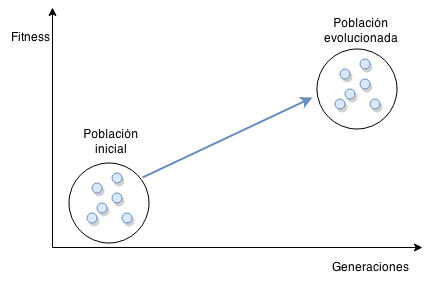
\includegraphics[width=10cm]{Figures/fitness_generaciones}
	\caption[Esquema de la evolución del valor del fitness en un algoritmo evolutivo ]{Esquema de la evolución del valor del fitness en un algoritmo evolutivo a través de las generaciones.}
	\label{fig:fitness_generaciones}
\end{figure}

Por tanto se van seleccionando, combinando y cambiando las mejores soluciones en un proceso, que si el AG está bien diseñado, permite ir obteniendo mejores soluciones.
El criterio de parada nos indica cuando termina este proceso, ya sea por que se alcanzó un número de generaciones predefinidos o por que la mejora no es evidente. Al final se devuelve la mejor solución encontrada en todo el proceso.

%Hay que indicar que no es una técnica exacta pero logra muy buenas aproximaciones, además se aplica en problemas complejos por su flexibilidad y robustez. 

A continuación se presentan las principales características de los AG.

\subsubsection{Esquema del algoritmo}

El esquema básico de funcionamiento se presenta en el Algoritmo \ref{alg:algoritmo_genetico_simple}:


\begin{algorithm}[H]
	\caption{Algoritmo Genético}
	\label{alg:algoritmo_genetico_simple}
	\begin{algorithmic} [1] 
		{
			%\small
			\STATE {Inicializo( Pob(0))}
			\STATE \texttt{generacion} = 0
			\WHILE {\text{No llegue al criterio de parada}}
			\STATE {Evaluar Pob(generacion)}
			\STATE {Padres = Seleccionar(Pob(generacion))}
			\STATE {Hijos = Cruzamiento(Padres) y Mutacion(Padres)}
			\STATE {NuevaPob = Reemplazar Pob(generacion) con Hijos}
			\STATE \texttt{generacion}++
			\ENDWHILE
			\RETURN Mejor solución
		}
	\end{algorithmic}
\end{algorithm}



\subsubsection{Representación de soluciones}
%Dado que no se puede trabajar directamente sobre las soluciones, estas se codificaron en un modelo donde es posible aplicar el algoritmo.
Los AG no trabajan directamente sobre las soluciones del problema, sino que utilizan una abstracción de las soluciones llamada cromosoma. Un cromosoma es un vector de genes donde el valor de cada gen se denomina alelo; nombres inspirados en la evolución natural biológica.
En general los AG codifican las soluciones utilizando un vector de números binarios o reales de largo fijo.

\begin{figure}[H]
	\centering
	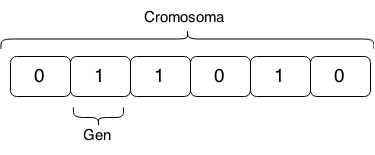
\includegraphics[width=8cm]{Figures/rep_binaria}
	\caption{Representación binaria de un cromosoma.}
	\label{fig:rep_binaria}
\end{figure}


\subsubsection{Función de Evaluación} 
La función de evaluación indica qué tan bueno es un individuo para resolver el problema en cuestión, utilizando un valor conocido como \emph{fitness}, por lo que también es llamada función de \emph{fitness}. Este valor se utiliza para definir cuales son los mejores individuos y de esta forma guiar la exploración hacia la región que incluya las mejores soluciones. En general, la función de fitness es la que consume la mayor cantidad de tiempo del algoritmo genético, en comparación con los demás operadores.

\subsubsection{Operador de Selección}
Existen diversos operadores de selección, cuya función es mantener las mejores características de los individuos en las siguientes generaciones. Entre ellos se encuentran:
\begin{itemize}
	\item Selección proporcional: Elige aleatoriamente individuos donde la probabilidad de selección es proporcional al valor del \emph{fitness}. Los mejores individuos son elegidos con mayor probabilidad, pero los peores individuos también pueden ser elegidos, lo que permite mantener la diversidad en la población. Sea N la cantidad de individuos en la población y $f_i$ el valor de \emph{fitness} del i-ésimo individuo, la probabilidad asociada a su selección esta dada por la la ecuación \ref{eq:seleccion_proporcional} .
	\item Torneo: Se eligen aleatoriamente un determinado número de individuos y se selecciona un subconjunto de los individuos con mejor \emph{fitness}.
	\item Rango: Se ordenan los individuos por el valor de \emph{fitness} y se selecciona un determinado porcentaje(rango) de los mejores individuos.
\end{itemize}

\begin{equation}
\label{eq:seleccion_proporcional}
F(x) =  p_i = \frac{f_i}{\sum_{j=1}^{n}{f_j}}  
\end{equation}
        
        
\subsubsection{Operador de cruzamiento}
La función del operador de cruzamiento es combinar individuos con el objetivo de preservar las mejores características de los progenitores y así lograr construir mejores soluciones. El operador de cruzamiento se aplica de acuerdo a una tasa de probabilidad prefijada. 

\begin{figure}[H]
	\centering
	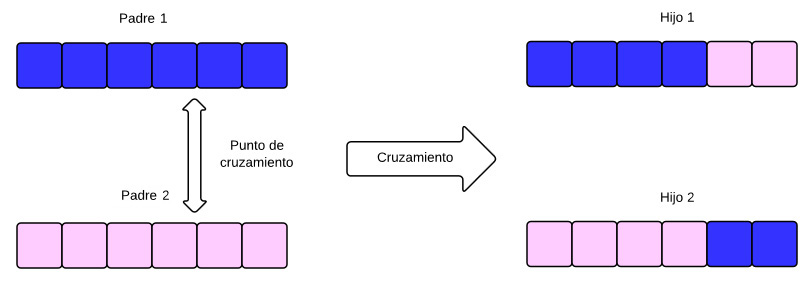
\includegraphics[width=\textwidth]{Figures/cruzamiento1}
	\caption{Cruzamiento de un punto}
	\label{fig:cruzamiento1}
\end{figure}

En general, los operadores de cruzamiento se pueden clasificar en:

\begin{itemize}
	\item Cruzamiento de un punto: A partir de dos padres se selecciona un punto al azar de los cromosomas obteniendo dos trozos que se combinan para obtener dos hijos. Se explica en la Figura ~\ref{fig:cruzamiento1}
	\item Cruzamiento multipunto: El método anterior se puede generalizar para obtener más puntos de corte y más recombinaciones.
	\item Cruzamiento uniforme: Para cada posición en el cromosoma se   intercambian genes según una tasa de probabilidad, este mecanismo se muestra en la Figura \ref{fig:cruzamiento_uniforme} .	
\end{itemize}



\begin{figure}[H]
	\centering
	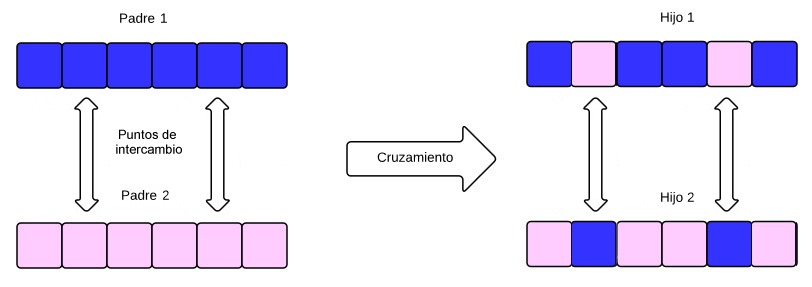
\includegraphics[width=\textwidth]{Figures/cruzamiento_uniforme}
	\caption{Cruzamiento uniforme}
	\label{fig:cruzamiento_uniforme}
\end{figure}

\subsubsection{Operador de mutación} 
El operador de mutación es el método utilizado para modificar un individuo, con el objetivo de mantener y mejorar la diversidad y otorgar al AG un mecanismo que le permita escapar de óptimos locales. En general la mutación aplica una modificación aleatoria en el cromosoma, por ejemplo, en una representación binaria se invertiría aleatoriamente el valor de un alelo, como se muestra en la Figura \ref{fig:mutacion1}.
\begin{figure}[h]
	\centering
	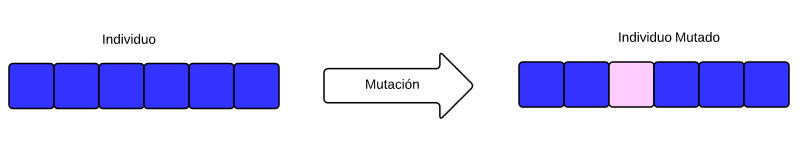
\includegraphics[width=1\linewidth]{Figures/mutacion1}
	\caption{Mutación por inversión binaria}
	\label{fig:mutacion1}
\end{figure}


\subsubsection{Criterio de reemplazo} 
Luego de que se aplica el cruzamiento se insertan nuevos individuos que aumentan la población original. Por lo tanto el operador de reemplazo indica cual es el criterio que se debe tomar para crear una nueva población con una cantidad de individuos igual a la original.
Se podría reemplazar todos los padres por los hijos, o seleccionar cuales reemplazar, entre otros criterios.

\subsubsection{Criterio de parada} 
El criterio de parada indica cuándo debe terminar el algoritmo. Puede definirse un número fijo de generaciones o determinar si el mejor valor de fitness se mantiene relativamente constante durante un número determinado de generaciones entre otros criterios. El objetivo será encontrar un compromiso entre un buen resultado y un tiempo acorde de ejecución, ya que el algoritmo no arrojará un valor exacto sino una buena aproximación. 



% ctrl+t comenta
%\begin{algorithm}%[!ht]
%	\caption{Genetic Algorithm}
%
%	\begin{algorithmic} [1] 
%		{
%
%			\STATE {Init( Pop(0))}
%			\STATE \texttt{generation} = 0
%			\WHILE {\text{NOT Stop Criteria}}
%			\STATE {Evaluate Pop(generation)}
%			\STATE {Parents = Selection(Pop(generation))}
%			\STATE {Children = Crossover(Parents) and Mutation(Parents)}
%			\STATE {NewPop = Replace Pop(generation) with Children}
%			\STATE \texttt{generation}++
%			\ENDWHILE
%			\RETURN Best solution
%		}
%	\end{algorithmic}
%\end{algorithm}


\subsection{Algoritmos evolutivos multiobjetivo}

Los problemas de optimización multiobjetivo trabajan sobre un espacio multidimensional de funciones y no tienen una única solución. Por este motivo, el significado de óptimo cambia. Una solución es un \emph{óptimo de Pareto} si ninguna de las funciones objetivo puede mejorar su valor sin degradar otro de los valores objetivo. Todas estas soluciones son consideradas igualmente buenas, ya que los vectores no se pueden ordenar completamente y representan diferentes valores de compromiso entre las funciones objetivo. Al conjunto de los valores funcionales de los óptimos de Pareto se les llama frente de Pareto.

Existen algoritmos evolutivos para resolver problemas de optimización multiobjetivo. 
Éstos son los llamados MOEA, por sus siglas en inglés \emph{ MultiObjetive Evolutionary Algorithm}. Sus propósitos son aproximarse al frente de Pareto y lograr obtener una gama de diferentes compromisos entre las funciones a optimizar para luego poder tomar la decisión de cual elegir.Para un análisis más detallado de los AE multiobjetivo se recomienda el trabajo de \citet{Deb2001}.


\begin{algorithm}%[!ht]
	\caption{Algoritmo Evolutivo MultiObjetivo. En rojo se indican las diferencias con el algoritmo evolutivo genérico.}
	\label{alg:algoritmo_genetico_multiobjetivo}
	\begin{algorithmic} [1] 
		{
			%\small
			\STATE {Inicializo( Pob(0))}
			\STATE \texttt{generacion} = 0
			\WHILE {\text{No llegue al criterio de parada}}
			\STATE {Evaluar Pob(generacion)}
			\STATE {\textcolor{red}{Operador Diversidad (Pob(generacion))}}
			\STATE {\textcolor{red}{Asignar Fitness (Pob(generacion))}}
			\STATE {Padres = Seleccionar(Pob(generacion))}
			\STATE {Hijos = Cruzamiento(Padres) y Mutacion(Padres)}
			\STATE {NuevaPob = Reemplazar Pob(generacion) con Hijos}
			\STATE \texttt{generacion}++
			\ENDWHILE
			\RETURN 	{\textcolor{red}{Frente de Pareto}}
		}
	\end{algorithmic}
\end{algorithm}

El Algoritmo \ref{alg:algoritmo_genetico_multiobjetivo} describe el esquema básico de un MOEA, donde se aprecia que existen dos operadores característicos: el operador de diversidad y el operador de asignación de \emph{fitness}. El primero se aplica para evitar la convergencia a un sector en particular del frente de Pareto, mientras que el segundo intenta brindar mayor chance de perpetuar a los individuos con mejores características.

Los MOEA se pueden clasificar por el método de asignación de fitness. Por un lado se tienen los que no son basados en Pareto, que utilizan métodos sencillos de asignación de fitness y son adecuados cuando el problema tiene no más de tres funciones objetivo. Un mecanismo popular entre los que no utilizan dominancia de Pareto es la combinación lineal de los objetivos. Por otro lado, los metodos de asignacion de fitness que se basan en Pareto dominancia de PAreto utilizan explícitamente la dominancia de Pareto al asignar el fitness.




\subsection{Algoritmos evolutivos paralelos}
Los problemas complejos suelen requerir una alta demanda computacional, por lo que paralelizar el algoritmo evolutivo es útil para lograr tiempos de ejecución menores. Pero este no es el único objetivo que se puede conseguir con un AE paralelo, entre otros existen: encontrar soluciones alternativas al mismo problema, búsqueda más eficiente aún sin \emph{hardware} paralelo, facilidad en la cooperación con otros métodos y búsqueda paralela de múltiples puntos en el espacio \citep{Alba2002}. 

En el caso de los algoritmos genéticos, gran parte del tiempo se ocupa en la etapa de evaluación de \emph{fitness}, por esta razón es un buen método distribuir la carga en varios procesadores para que las evaluaciones se realicen en paralelo. 

Un modelo muy utilizado es el \emph{maestro-esclavo}. El proceso maestro es el encargado de ejecutar los operadores básicos del algoritmo y distribuir a procesos esclavos la evaluación de la función fitness para un conjunto de individuos. El esclavo devuelve el resultado y luego el maestro es el encargado de continuar con la evaluación, ejecutando los operadores. De este modo aumenta la eficiencia computacional del algoritmo ya que una de las funciones más costosas es distribuida entre varios procesos que ejecutan concurrentemente.

\begin{figure}[H]
	\centering
	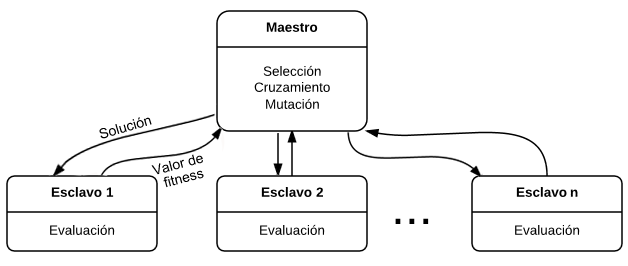
\includegraphics[width=0.9\linewidth]{Figures/diagrama-master-slave}
	\caption[Modelo Maestro-Esclavo]{Modelo Maestro-Esclavo}
	\label{fig:diagrama-master-slave}
\end{figure}

\subsection{Implementación y entornos de desarrollo}

A la hora de implementar un algoritmo genético es importante tener en cuenta ciertos aspectos que dotarán a la solución de una mayor flexibilidad, eficiencia y robustez. En general se recomienda usar el paradigma de orientación a objetos, ya que aporta múltiples ventajas entre las que se encuentra: reusabilidad del código, abstracción de problemas, modularidad y legibilidad. Sin embargo, la orientación a objetos esto puede ocasionar pérdidas de eficiencia computacional, por lo que hay que balancear estos aspectos.

En el trabajo de \citet{Alba1997} se indican con más detalle los elementos importantes de una implementación de AG, entre ellas se destacan: no utilizar tamaño fijo para las poblaciones pues afectan la flexibilidad, evitar las múltiples evaluaciones de una misma solución, dar al usuario la posibilidad de extender las funcionalidades de manera modular, al implementar bibliotecas genéricas usar lenguajes orientados a objetos que permiten su extensión en forma sencilla. Por estas razones se han desarrollado entornos de desarrollo o\emph{frameworks} para trabajar en la resolución de problemas utilizando algoritmos evolutivos y otras técnicas metaheurísticas. Los \emph{frameworks} encapsulan de manera transparente al usuario los aspectos antes mencionados, lo que permite un desarrollo más rápido, sencillo y seguro.

Existe una gran variedad de \emph{frameworks} para AE; a continuación se describen algunos de los más populares junto con sus principales características.

\begin{itemize}
	\item JMetal: Es un \emph{framework} orientado a objetos basado en Java para la resolución de problemas de optimización multiobjetivo utilizando metaheurísticas. Su arquitectura permite experimentar con técnicas embebidas y también desarrolladas por el usuario. Entre sus características destacan que al estan implementado en Java puede ser usado tanto en sistemas Windows como Linux. Posee una amplia variedad de algoritmos multiobjetivo listos para usar, y también algoritmos paralelos. Está en constante desarrollo y posee una documentación detallada \citep{Jmetal}.
	
	\item Galib: Es una biblioteca escrita en C++ que incluye objetos y herramientas útiles para la resolución de problemas usando algoritmos genéticos. Es gratuita y de código abierto, pudiendo ser ejecutada tanto en Linux como en Windows. No tiene un desarrollo sostenido, siendo su última actualización en el año 2000, esto no quita que todavía se siga usando por su sencillez y flexibilidad \citep{Galib}.
	
	\item Paradiseo: Es un \emph{framework} orientado a objetos que utiliza C++. Su objetivo es el diseño de metaheurísticas tanto paralelas como distribuidas. Cuenta con algoritmos evolutivos, búsquedas locales y optimización basada en enjambres. Funciona tanto en plataformas Windows como Linux y posee varios módulos destinados a extender sus funcionalidades. Tiene una buena documentación y su ultima versión data del año 2012 \citep{Paradiseo}.
	
	\item Open Beagle: Es un \emph{framework} en C++ utilizando algoritmos evolutivos. Brinda un entorno de alto nivel para trabajar con distintas técnicas, soportando programación evolutiva, algoritmos genéticos y estrategias evolutivas. Su arquitectura permite utilizar los principios de la programación orientada a objetos para lograr un código recusable y eficiente. Sus características apuntan a brindar un entorno amigable, eficiente, multi-plataforma y gratuito \citep{OpenBeagle}.
	
	\item Mallba: Es una biblioteca escrita en C++ que brinda esqueletos de algoritmos exactos, metaheurísticas, e híbridos para la resolución de problemas de optimización. Mallba maneja el paralelismo de forma simple para el usuario. Posee una arquitectura flexible y extensible lo que permite agregar nuevos esqueletos de forma simple. No cuenta con documentación extensa pero si con varios ejemplos completos de implementaciones de los algoritmos. Mallba funciona tanto en ambiente Linux como Windows \citep{Mallba}.
	
	\item Malva: Surge como un \emph{branch} de la biblioteca Mallba, con modificaciones para ser ejecutado en ambientes actuales, por lo que cuenta con las mismas características aunque al estar en fase de desarrollo soporta solo algunos algoritmos, entre ellos algoritmos genéticos \citep{Malva}.
\end{itemize}

Los \emph{frameworks} son una herramienta importante a la hora de desarrollar un algoritmo evolutivo. Al enfocarse en el problema de la sincronización de semáforos también serán necesarias otras utilidades entre las que se encuentra los simuladores de tráfico, los cuales serán explicados en la siguiente sección.


\section{Simulación de tráfico}

Los simuladores de tráfico son programas que simulan el movimiento del flujo vehicular sobre una red terrestre, marítima o aérea. Son usados en proyectos de investigación, estudio de congestiones y análisis de impacto de obras.  Existen varias razones para optar por esta herramienta, entre las que se encuentra: la rapidez en la obtención de resultados y el costo asociado de implementación.

% la rapidez en la obtención de resultados ya que la simulación se puede realizar en tiempos mucho más rápidos que en la realidad, el costo, pues no es necesario cambiar la infraestructura para probar nuevos escenarios y es útil para prever situaciones que podrían darse bajo determinadas circunstancias.

Los simuladores se pueden dividir en dos grandes categorías, macroscópicos y microscópicos. En algunos casos se considera una tercera categoría híbrida de estas dos llamada mesoscópicos. En los simuladores \emph{macroscópicos} el tráfico es modelado como un flujo continuo y es descrito de manera agregada usando características como la velocidad o densidad del flujo. En los simuladores \emph{microscópicos} el tráfico se considera compuesto de partículas discretas. Cada partícula es actualizada según las propiedades de la red en ese momento, como limites de velocidad, vehículos cercanos y caminos a seguir. Los simuladores microscópicos utilizan un modelo de decisiones del conductor, lo que permite crear una distribución heterogénea del comportamiento de los vehículos. En general, los simuladores \emph{mesoscópicos} representan a los individuos con alto nivel de detalle pero sus interacciones y actividades con un bajo nivel de detalle, por ejemplo, agrupando vehículos en paquetes que se mueven por una red, considerándolos como una sola entidad.


Se considera que las simulaciones microscópicas se aproximan más a la realidad y que obtienen un nivel de granularidad mayor. Estas características pueden ser útil cuando se asignan propiedades sobre cada vehículo y se quiere observar el comportamiento cuando éstas cambian. Sin embargo, no implica que se dejen de usar simulaciones macroscópicas pues aunque no poseen tanto detalle si son más rápidas y en determinadas circunstancias podrían ser una mejor opción.

En la actualidad existe una gran variedad de simuladores disponibles, que se encuentran en las diferentes categorías que fueron mencionadas anteriormente. A continuación se ofrece una breve descripción de alguno de los simuladores presentados en el trabajo de \citet{review_trafico} que presenta una lista detallada de simuladores de tráfico.
\begin{itemize}
	\item SUMO: Simulador abierto, portable, microscópico diseñado para soportar grandes redes de tránsito. Es de los más populares, y utiliza una serie de archivos de configuración para representar las rutas, los vehículos y el tráfico \citep{SUMO}.
	\item QuadStone Paramics Modeller: Simulador modular y microscópico capaz de modelar un amplio rango de problemas de tránsito y transporte.
	\item Aimsun: Paquete de simulación que integra varios tipos de modelos de transporte, por ejemplo herramientas para el tráfico estático y un simulador microscópico
	\item Trafficware SimTraffic: Es un simulador que forma parte del paquete \emph{Trafficware's Syncro Studio}, que cuenta con una herramienta para la sincronización de semáforos.
	\item Corsim Trafvu: Parte del paquete \emph{Tsis Corsim}, presenta las animaciones y los gráficos estáticos para las redes de tráfico utilizando \emph{Corsim} como entrada.
\end{itemize}

Cabe destacar que de los cinco simuladores de tráfico mencionados anteriormente, solamente SUMO es abierto y gratuito, el resto son programas propietarios. 

\begin{figure}[H]
	\centering
	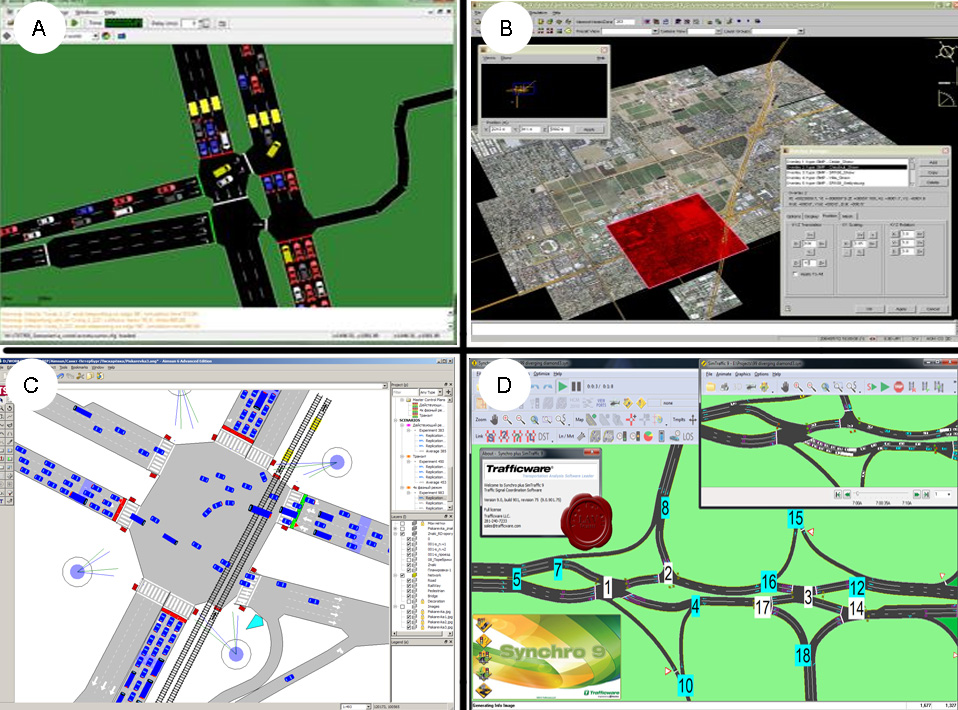
\includegraphics[width=0.9\linewidth]{Figures/simuladores}
	\caption[]{Algunos simuladores de tráfico. (A) Sumo, (B) QuadStone Paramics, (C) Aimsun, (D) Trafficware SimTraffic}
	\label{fig:simuladores}
\end{figure}

Los simuladores requieren de la creación de una \emph{red de tránsito}. En general, la red refiere a las propiedades que tendrán las vías de tránsito, por ejemplo la cantidad de carriles, el limite de velocidad, la ubicación, el largo, las conexiones entre calles, etc. Algunos simuladores obtienen ésta entrada desde archivos de texto, lo cual puede ser un proceso lento y propenso a errores; otros pueden importar redes viales de servicios, como Open Street Map \citep{OSM}. También necesitan conocer las\emph{ rutas seguidas por los vehículos}. Los simuladores pueden tomar esta información de manera explicita, indicando para cada vehículo la ruta seguida, o utilizar otros métodos dinámicos indicando sólo los puntos de inicio y final del recorrido, cuya ruta será generada en tiempo de simulación. El procesamiento manual para generar los recorridos vehiculares puede ser un proceso verdaderamente complejo, por este motivo muchos simuladores brindan herramientas destinadas a facilitar esta tarea.

Un aspecto importante a tener en cuenta es la salida que genera el simulador, ya que es fundamental a la hora de analizar resultados y sacar conclusiones. En general, la información básica reportada incluye: la velocidad y tiempos de recorrido, aunque también puede contener más detalles incluyendo: la duración de detenciones, la densidad de tráfico, uso de combustible y/o la cantidad de emisiones contaminantes.  
 
\section{Trabajos relacionados}

La investigación del estado del arte se realizó con dos objetivos en mente, el primero fue analizar las distintas soluciones que existen actualmente para el problema de sincronización de semáforos y el segundo fue para encontrar nuevas prácticas, algoritmos o utilidades que pudieran fortalecer la solución a implementar.

El problema del tráfico optimizando las luces de los semáforos se puede resolver por diferentes métodos incluyendo  redes neuronales \citep{Lopez1999}, lógica difusa \citep{Lim2001}, redes de petri \citep{DiFebbraro2002}, entre otros. El número de artículos encontrados en el relevamiento de trabajos relacionados fue abundante y los tipos de propuesta fueron variadas, por este motivo se decidió enfocar la búsqueda en los trabajos que proponen soluciones cercanas al proyecto propuesto. En particular se relevaron aquellos trabajos que utilizan algoritmos genéticos.

Una reseña de los principales trabajos relacionados se presenta a continuación:


\begin{itemize}
\begin{item}
\bibentry{Sanchez2004}

  
Este trabajo se basa en tres ideas fundamentales: El uso de algoritmos genéticos para la sincronización de los semáforos, la simulación de autómatas celulares para la función de evaluación del tráfico y un cluster para realizar ejecuciones del algoritmo en paralelo.
El caso de estudio presentado es pequeño, con 5 calles de 2 vías que se intersectan. La codificación del cromosoma utiliza un vector de números enteros, donde se codifica para cada intersección cuál es la calle habilitada en cada ciclo. El AG utiliza una estrategia de selección elitista, donde los dos mejores individuos se clonan a la siguiente generación y el resto son generados aplicando un operador de cruzamiento de dos puntos.

Para la evaluación del \emph{fitness}, se considera el tiempo que transcurre desde el momento en que un vehículo entra en la red hasta que sale. Se ejecuta sobre un cluster en forma paralela con una estrategia maestro-esclavo. El maestro envía los cromosomas a los esclavos para que evalúen y devuelven el resultado, luego el maestro se encarga de generar la siguiente población.
Se comparan los resultados obtenidos por el algoritmo con una simulación aleatoria y con una fija, obteniendo la solución propuesta mejores resultados en todos los casos evaluados.
	
El mismo grupo de trabajo realizaron otros similares, expandiendo esta investigación, los cuales se presentan a continuación.
\end{item}
	
\begin{item}
\bibentry{Sanchez2008}

Este estudio aplica lo presentado en el trabajo anterior a un escenario real en Santa Cruz de Tenerife. Algunas mejoras introducidas en el modelo del problema incluyen una nueva codificación del cromosoma utilizando código de Gray, que según los autores permite mejorar el desempeño computacional de los operadores de mutación y cruzamiento. La población inicial se compone de nueve soluciones provistas por la alcaldía de la ciudad. Las estrategias de selección, cruzamiento y mutación son similares a las aplicadas en el trabajo anterior.

El escenario discretizado de la zona estudiada lo componen 42 semáforos, 26 vías de entrada y 20 de salida. Las soluciones provistas por la alcaldía se ejecutaron en el simulador y los resultados obtenidos se compararon con los valores alcanzados  por el algoritmo, concluyendo que logra una mejora de 26\% en el valor del fitness.

\end{item}

\begin{item}
\bibentry{Sanchez2010}

Este trabajo contiene puntos de contacto con el presentado anteriormente. Un cambio introducido fue el análisis de cuatro funciones de fitness diferentes, evaluando: \textit{i)} la cantidad de vehículos que llegaron a destino, \textit{ii)} el tiempo de viaje promedio, \textit{iii)} el tiempo de ocupación promedio y \textit{iv)} la velocidad promedio global. 

El trabajo incorpora nuevas métricas correspondientes al gas total emitido por los vehículos, que tienen relación con la velocidad a la que circulan. El modelo discretizado de la zona de \emph{La Almozara} cuenta con 17 semáforos, 7 intersecciones, 16 entradas y 18 salidas. El análisis experimental incluye 10 escenarios que van desde baja congestión de trafico hasta alta. Se analizan los resultados para las distintas funciones de fitness concluyendo que las mayores mejoras en el valor de \emph{fitness} ocurren cuando la congestión de tráfico es más alta.

\end{item}


\begin{item}
\bibentry{Penner2002}

Este trabajo se centra en un modelo de simulación basado en enjambres. Utiliza un algoritmo genético con el objetivo de sincronizar los semáforos y así minimizar el tiempo de espera de los vehículos en toda la red vial. El cromosoma contiene la secuencia y duración de los semáforos, así como la relación con los semáforos complementarios. La mutación tiene en cuenta esa relación para no generar inconsistencias, por ejemplo: que ocurran dos luces verdes en la misma intersección. Existe mayor probabilidad de cruzamiento entre semáforos que se encuentran en la misma intersección. La función de \emph{fitness} calcula la relación entre el tiempo total de viaje y el tiempo de espera de todos los vehículos. 

El primer escenario considerado en el análisis experimental es pequeño; cuenta con una ruta de tres carriles y tres intersecciones. En este escenario el AG logra mejoras significativas. Luego se resuelve un segundo escenario más complejo, de 28 semáforos y 9 intersecciones, logrando mejoras de hasta 26\% en el tiempo de espera total.
\end{item}	


\begin{item}
\bibentry{Stolfi2012}

Este trabajo propone el concepto de ciudad inteligente, enfocado en la movilidad, indicando que la congestión de tráfico provoca tanto pérdidas económicas como contaminación ambiental. Plantea el desarrollo de un algoritmo inteligente, que toma en cuenta el estado de congestión de las rutas y sugiere al usuario la ruta más rápida a su destino con el objetivo de minimizar los tiempos de viaje de los vehículos que circulan por la red vial. Para detectar el nivel de congestión, utiliza un dispositivo en el automóvil que se enlaza por \emph{wifi} con los semáforos, los cuales cuentan con sensores. El trabajo no se basa en la sincronización de los semáforos, sino que presenta un sistema de búsqueda de la mejor ruta.

El escenario experimental presentado incluye una zona de la ciudad de Málaga, que cuenta con ocho entradas y ocho salidas. Para la simulación del tráfico utiliza el simulador SUMO. Los vehículos modelados son: turismo, monovolumen, furgoneta y camión. Cada vehículo del modelo posee características diferentes como: la longitud, velocidad y probabilidad que entre en la red de tráfico.

 Implementa un algoritmo genético, donde los cromosomas representan los sensores, que incluyen la información de los destinos y rutas posibles. La estrategia de selección consiste en tomar los dos peores individuos y reemplazarlos por los dos mejores hijos encontrados. La función de \emph{fitness} tiene en cuenta los valores obtenidos de la simulación del trafico, incluyendo: la cantidad de viajes completados, el tiempo medio de viaje y el retraso medio. 

Para el análisis experimental, obtiene los resultados bases simulando 64 itinerarios diferentes y los compara con la aplicación del algoritmo inteligente. Las simulaciones se realizan hasta con 800 vehículos, concluyendo que al aumentar la cantidad de vehículos (más de 400) en el sistema, el algoritmo mejora sustancialmente los resultados bases.

\end{item}	


\begin{item}
\bibentry{Teo2010}

Este trabajo presenta un escenario simple de una intersección donde un algoritmo genético intenta optimizar los tiempos de las luces de los semáforos para lograr mejorar el tráfico vehicular. El cromosoma representa los tiempos de la luces verdes, mientras que la función de \emph{fitness} se calcula teniendo en cuenta el largo de las colas generadas por los vehículos en las intersecciones. La ejecución de la simulación utiliza un tiempo fijo de 600 segundos por generación, pero no se describe el tipo de simulador utilizado. El análisis experimental compara los resultados del AG cuando el escenario tiene en cuenta un flujo continuo de vehículos, y cuando no. Entre las conclusiones del trabajo se indica, que la optimización de las luces de los semáforos usando algoritmos genéticos es una buena opción para resolver el problema de la congestión del tráfico.	
\end{item}	


\begin{item}
\bibentry{Montana1996}

Esta propuesta utiliza un enfoque adaptativo, con sensores que analizan el tráfico en tiempo real. Un sensor contabiliza los autos que circulan y otro detecta el largo de la cola de vehículos generada en la intersección. Se consideran los cambios producidos respecto al caso promedio y se modifican los tiempos de las luces de los semáforos de forma acorde, con el objetivo de mejorar la circulación del tránsito. 

Se aplica un algoritmo híbrido entre programación genética, específicamente STGP (strongly typed genetic programming) \citep{Montana1995} y un algoritmo genético, para resolver el problema de sincronización se semáforos. La medida básica de efectividad en la función de evaluación es el \emph{delay}, que representa el total de tiempo perdido causado por las señales de tráfico. 

El análisis experimental se desarrolló es un escenario simple con cuatro intersecciones y tres tipos de tráfico diferente, utilizando una versión especial del simulador TRAF-NETSIM \citep{TRAF-NETSIM}. En los experimentos se comparan los valores obtenidos utilizando una configuración fija de los semáforos, cuyos valores fueron obtenidos al aplicar un AG, contra el algoritmo adaptativo desarrollado. Los resultados indican que se aprecian mejoras en el flujo de tránsito ( hasta 40 \% en el valor de \emph{fitness})  y destaca la buena adaptabilidad del algoritmo implementado en diferentes circunstancias. Sin embargo, recalca que el escenario es simple y de tamaño reducido, siendo una incógnita como el algoritmo funcionará en problemas más complejos.

\end{item}	


\begin{item}
\bibentry{Vogel2000}

Este trabajo utiliza un enfoque auto-adaptativo para mejorar el tráfico, tanto en el corto como en el largo plazo, a través de la optimización de las señales de tráfico en las intersecciones de una red de rutas. 

Presenta la idea de que una configuración de semáforos particular, aún siendo optimizada usando simulaciones, tiene poca probabilidad de ser la mejor en todas las situaciones o en casos extremos (horas picos). Para solucionar ese problema, propone un sistema auto-adaptable que toma la información del tráfico actual usando detectores de vehículos y espacios disponibles.

Propone el desarrollo de un algoritmo evolutivo donde cada individuo representa un sistema de fases de los semáforos, mientras la función de \emph{fitness} tiene en cuenta las demoras en el tráfico, que se obtiene utilizando simulaciones. El escenario es relativamente pequeño, con una intersección de dos calles, cada una con tres líneas, donde la ruta principal tiene el doble de densidad vehicular. Los resultados obtenidos de este trabajo indican que la ventaja de usar conocimiento experto para configurar los parámetros iniciales es mínimo, ya que el algoritmo llega rápidamente a resultados similares. No se realizaron comparaciones con otros escenarios, solo se estudió el comportamiento del algoritmo evolutivo utilizando diferentes parámetros..

\end{item}	

\begin{item}
\bibentry{Rouphail2000}

Este trabajo estudia una pequeña red de tráfico con nueve intersecciones semaforizadas en la ciudad de Chicago (USA); el escenario incluye: la red vial, el tráfico de vehículos,  y las paradas de ómnibus. Se toman valores reales de tráfico en horas pico, comprobando que las colas de vehículos generadas en la simulación coinciden con la realidad. Utiliza el programa \citet{TRANSYT-7F} que permite visualizar mapas y un simulador de tráfico comercial llamado \citet{CORSIM}. El objetivo es resolver el problema de sincronización de semáforos, utilizando un AG cuya función de evaluación que tiene en cuenta las demoras en la red y el largo de las colas producidas por los vehículos. El análisis experimental compara los valores de la realidad, con los resultados obtenidos por el AG. Los resultados indican que el AG mejora los valores del caso base, reduciendo las demoras simuladas en un 44\%.

\end{item}	
	
\end{itemize}


\subsection{Resumen}
Esta sección presenta un breve análisis sobre los trabajos evaluados y como se relacionan con el presente proyecto.

El trabajo de \citet{Sanchez2004} incluye algunos puntos de contacto con el presente proyecto, ambos utilizan un cluster como plataforma de ejecución del algoritmo evolutivo y aplican el mismo método de paralelismo (maestro-esclavo) en el modelo de paralelismo. La principal diferencia entre ambos trabajos, es que el escenario que evalúan es pequeño y no se realizan comparaciones con modelos que representen un escenario real. El siguiente trabajo de \citet{Sanchez2008} expande lo anterior y lo aplica a un escenario real, en Santa Cruz de Tenerife. Este escenario presenta una complejidad similar al Corredor Garzón en términos de cantidad de cruces y semáforos. Los resultados obtenidos son muy positivos, obteniendo mejoras de hasta 26\% en el valor de \emph{fitness}.

Se destaca de \citet{Sanchez2010} las pruebas realizadas con diferentes funciones de \emph{fitness}, teniendo en cuenta diversos factores como: tiempo de viaje o velocidad promedio. Este trabajo inspiró al presente proyecto en considerar la realización de una función multiobjetivo que tuviera en cuenta la velocidad promedio de los autos y ómnibus.

En el trabajo de \citet{Stolfi2012} no se optimiza la configuración de los semáforos, pero plantea una posibilidad interesante para mejorar el tráfico de una ciudad indicando a los conductores la mejor ruta a seguir. Esta novedosa opción se podría tomar como un elemento en trabajos futuros. Tanto \citet{Teo2010} como \citet{Stolfi2012} plantean la simulación con un tiempo fijo, característica que se consideró para el presente proyecto.

\citet{Montana1996} y \citet{Vogel2000}  proponen algoritmos adaptables en tiempo real, siendo un aporte interesante a tener en cuenta para trabajos a futuro.

En conclusión, el estudio de los trabajos relacionados permitió conocer en profundidad distintas soluciones y métodos que se consideraron en menor o mayor medida en la solución propuesta. El hecho de que todos los trabajos consultados obtuvieron mejoras significativas en sus resultados motivó aún más el desarrollo del presente proyecto.

\begin{table}[H]
	\renewcommand{\arraystretch}{1.2}
	\caption{Resumen de los principales trabajos relacionados relevados.}
	\label{table:resumen_trabajos}
	\centering
	\begin{tabular}{p{3cm}p{1cm}p{9cm}}
		\hline
		Autor& 
	    Año & 
		Línea de trabajo\\ 
		\hline
		\citeauthor{Montana1996} & \citeyear{Montana1996}   &  Sincronización de semáforos en tiempo real utilizando un algoritmo híbrido entre programación genética y  algoritmo genético en un escenario simple. \\
		\citeauthor{Vogel2000} & \citeyear{Vogel2000}       &  Sincronización de semáforos en tiempo real utilizando un algoritmo evolutivo un escenario simple.\\
		\citeauthor{Rouphail2000} & \citeyear{Rouphail2000} &  Sincronización de semáforos utilizando un algoritmo genético en un escenario real.\\			
		\citeauthor{Penner2002} & \citeyear{Penner2002}     &  Sincronización de semáforos utilizando un algoritmo genético en un escenario complejo.\\	
	    \citeauthor{Sanchez2004} & \citeyear{Sanchez2004}   &  Sincronización de semáforos utilizando un algoritmo genético en un escenario simple.\\
		\citeauthor{Sanchez2008} & \citeyear{Sanchez2008}   &  Sincronización de semáforos utilizando un algoritmo genético en un escenario real.\\
		\citeauthor{Sanchez2010} & \citeyear{Sanchez2010}   &  Sincronización de semáforos utilizando un algoritmo genético en un escenario real. Análisis de cuatro funciones de fitness diferentes.\\
		\citeauthor{Teo2010} & \citeyear{Teo2010}           &  Sincronización de semáforos utilizando un algoritmo genético en un escenario simple.\\
		\citeauthor{Stolfi2012} & \citeyear{Stolfi2012}     &  Propone el concepto de ciudad inteligente, utilizando un algoritmo genético para sugerir la mejor ruta a los conductores en tiempo real.\\


			
		\hline
	\end{tabular}
\end{table}









\chapter{Estrategia de resolución}


\section{Framework}

Malva [http://themalvaproject.github.io/] surge como un fork del proyecto Mallba [http://neo.lcc.uma.es/mallba/easy-mallba/index.html ] . Propone la actualización, mejora y desarrollarlo como un proyecto de código abierto colaborativo.  Su objetivo es proveer de varios esqueletos de heuristicas de optimización que puedan ser utilizados y extendidos de manera fácil y eficiente.

Los esqueletos se basan en separar dos conceptos: El problema concreto que se quiere resolver y por otro lado el método utilizado para resolverlo. Por tanto un esqueleto se puede ver como un template genérico que se instancia para resolver un problema particular, manteniendo todas las funcionalidades genéricas.

Utiliza el lenguaje c++ dado su alto nivel, modularidad y flexibilidad. Los esqueletos se ofrecen como un conjunto de clases requeridas que son las que el usuario deberá modificar para adaptarlo a su problema y las provistas. que incluyen todos los aspectos internos del esqueleto y on independientes dle problema particular.
Los esqueletos provistos o sea los algoritmos soportados son Algoritmos genéticos y CHC.




\section{Algoritmo Genético}
El algoritmo que vamos a utilizar es el algoritmo simple, este
sigue  la  propuesta  de  Goldberg  [].  El  algoritmo  en  Malva  se
llama NewGA, el mismo crea una población inicial y en
cada  generación,  genera  una  nueva  población  de  individuos
seleccionando  de  la  población  anterior  y  realizando
cruzamiento,  hace  un  reemplazo  total.  El  proceso  se  repite
hasta  dar  con  algún  tipo  de  criterio  de parada.  La  librería se
basa en el elitismo, los mejores individuos son llevados hacia
la siguiente generación.

\subsection{Representación}
Para poder explicar la representación del problema de los
semáforos del corredor Garzón, es preciso compartir algunas
definiciones que usaremos a lo largo de la propuesta:
Cruce: se define como el lugar de intersección de dos o
más vías de circulación.
Fase: es la configuración de las luces de los semáforos
en un determinado cruce; un cruce tiene hasta 8 fases.
Por ejemplo una fase de un cruce puede ser
“rrrrGGrrrrGG” durante 52 segundos. Donde “G” es
Verde, “r” es Rojo y “y” es Amarillo.  
Es  importante  que  el  algoritmo  evolutivo  a  implementar  no
genere soluciones que no sean viables por lo que éste no debe
de poder modificar la combinación de luces de cada fase y de

esta manera no se generarán fases con combinaciones de luces
equivocadas (podría generar accidentes de tránsito).
En  pos  de  un  mejor  rendimiento  y  ya  que  en  realidad  no
modifican  los  tiempos  reales  del  paso  de  los  vehículos,  se
omitieron  las   fases  que  tienen  luces  amarillas  en  la
representación del cromosoma.
El  cromosoma  se  va  a  agrupar  lógicamente  en  cruces,
definimos el valor de un gen como el tiempo que demora una
fases  de  un  cruce  (sin  considerar  las  amarilla,  estas  quedan
fijas con el valor obtenido en la realidad) o la fase con la que
inicia un cruce, por lo que el tamaño del cromosoma depende
de  la  cantidad  de  cruces  y  de  la  cantidad  de  fases  que  tiene
cada cruce, teniendo así la información de todos los cruces.

\subsection{Codificación} 
A continuación se muestra un ejemplo en el cual se mapea un
cruce representado en el cromosoma y un cruce representado
en  el  archivo  de  configuración  de  semáforos  que  utiliza  el
simulador SUMO.
Como se  mencionó anteriormente se omite el valor de la luz
amarilla en el cromosoma y se mantiene el valor real recabado
y el valor que tiene el cromosoma en el gen de inicio de fase
se corresponde con el valor de “offset” en el XML.
Cruce representado en el cromosoma:

\subsection{Inicialización}
Para la inicialización de la población se toma como referente
la configuración obtenida con los datos in situ, luego para cada
cruce  se  hacen  variar  las  duraciones  de  las  fases  de  manera
aleatoria  entre  un  rango  de  5  segundos  a  60  segundos  (estos
valores  son  configurables)  y  la  fase  inicial  se  hace  variar
aleatoriamente entre la cantidad de fases del cruce  (se cuentan
las luces amarillas).

\subsection{Función fitness}
Para evaluar un individuo, lo que se hace es crear un archivo
XML  de configuración de señalización de tránsito que utiliza
el  simulador  SUMO  en  base  al  cromosoma  del  individuo,
luego se ejecuta el simulador con la configuración generada, el
tiempo de simulación devuelto será el valor de la función de
fitness.

\subsection{Operadores}
\subsubsection{Selección}
\subsubsection{Cruzamiento}
Se  utilizará  cruzamiento  de  un  punto  (1PX),  implementado
específicamente  para  el  problema,  seleccionando  el  intervalo
entre 2 cruces como punto de corte, por ejemplo:
Esto  hace  que  si  un  tramo  del  corredor  es  bueno,  esta
propiedad se mantenga.

\subsubsection{Mutación}
La  mutación también fue  implementada  específicamente para
el problema, utilizaremos dos tipos de mutación:
Mutación de duración de fase: para cada fase de cada cruce se
hace variar su duración sumando o restando una cantidad dada
de segundos entre un rango determinado con una probabilidad
dada.
Mutación de inicio de cruce: se elige aleatoriamente una fase
con  la  cual  va  a  arrancar  inicialmente  el  cruce  con  una
probabilidad dada.

\subsection{Criterio de parada}
 Cantidad  de  generaciones:  Es  la  cantidad  de
 generaciones  con  la  cual  se  toma  el  criterio  de  parar  la
 ejecución del algoritmo, el número de generaciones que vamos
 a usar es 100.
 Probabilidad  de  convergencia:  La  convergencia  se
 define como la relación entre los N mejores valores de fitness
 de  las  generaciones  anteriores  contra  el  mejor  valor  de  la
 generación actual. Nosotros vamos a utilizar N con el valor de
 10 y una probabilidad de convergencia de 0.99




\section{Multiobjetivo}

\section{Algoritmo Paralelo}
Agregar diagrama de maestro esclavo



\section{Resumen}
\chapter{Análisis Experimental}
Esta sección presenta la evaluación experimental del Algoritmo Evolutivo multiobjetivo propuesto para resolver el problema de sincronización de semáforos del corredor Garzón. Inicialmente se presenta una descripción de los escenarios utilizados en la evaluación experimental y la plataforma de ejecución en la que se llevo a acabo la experimentación. A continuación se detalla el análisis experimental, que se divide en dos etapas: primero se analiza la configuración paramétrica para encontrar una mejor calidad de resultados y luego se realizan los experimentos de validación para los que se reportan los resultados numéricos. Finalmente se presentan un breve análisis de la eficiencia computacional lograda por el algoritmo.



\section{Plataforma de ejecución y Desarrollo}
Como se explicó en el capitulo anterior se utiliza el algoritmo genético provisto por la biblioteca Malva que fue extendida en el código base para soportar la creación de nuevos hilos de ejecución para lograr el funcionamiento en paralelo.

Dada la complejidad del problema el análisis experimental  se realiza en la plataforma Cluster Fing (sitio web: http://www.fing.edu.uy/cluster) para poder acelerar el tiempo real de procesamiento al ejecutar el algoritmo en paralelo distribuyendo la carga en varios núcleos. Específicamente fue utilizado un procesador AMD Opteron 6272 de 2.09GHz, 48Gb RAM, 64 núcleos, corriendo el sistema operativo CentOS Linux 6.5.

Las pruebas incluidas en el análisis experimental utilizaron entre 4 y 32 procesadores ya que por la naturaleza de recursos compartidos no siempre se tiene una cantidad igual de procesadores libres y para la mayoría de las pruebas el número de procesadores no es relevante. Si lo será cuando se realice el análisis de eficiencia computacional que se estudiará más adelante.


\section{Ajuste paramétrico}
En vez de utilizar valores fijos para los parámetros, se realiza un análisis para determinar el mejor valor para cada parámetro usado en el algoritmo evolutivo propuesto. Esto tiene como objetivo obtener una mejor calidad de resultados. Los parámetros que se ajustan son el \emph{tiempo de simulación} que se refiere al parámetro del simulador SUMO para determinar la duración de la simulación. Luego el parámetro de \emph{criterio de parada} indica el método usado para detener el algoritmo y el \emph{tamaño de la población} que representa la cantidad de individuos que tiene la población utilizada en el algoritmo evolutivo. Finalmente se ajustan los parámetros de la \emph{probabilidad de mutación y la probabilidad de cruzamiento}. Todos estos parámetros serán tratados en detalle en las siguientes subsecciones.

Se generan tres escenarios de tráfico diferentes, que serán utilizados en el ajuste de cada parámetro. En este caso no se utilizan datos recabados de la realidad, como el tráfico vehicular o la frecuencia de los ómnibus, para no sesgar el algoritmo a un caso en particular.
A continuación se presenta la cantidad de vehículos para cada uno de los tres escenarios de tráfico propuestos:

\begin{itemize}
	\item Tráfico Bajo: 30 ómnibus y 500 vehículos	
	\item Tráfico Medio: 60 ómnibus y 1000 vehículos
	\item Tráfico Alto: 120 ómnibus y 2000 vehículos
\end{itemize}


En el ajuste paramétrico primero se define el tiempo de simulación, el criterio de parada y el tamaño de población. Luego de establecidos los valores para los parámetros mencionados, se realizan las pruebas para todas las combinaciones de probabilidad de cruzamiento y mutación buscando los mejores valores para ajustar el algoritmo.

La plataforma Cluster Fing donde se desarrolla el análisis experimental permite disponer tanto de la métrica del tiempo real que dura la ejecución, así como también el tiempo secuencial, es decir la suma del tiempo de procesamiento de todos los procesadores involucrados en la evaluación del algoritmo. Cuando se realizan comparaciones en los tiempos de ejecución se utiliza el tiempo secuencial que es independiente de la cantidad de procesadores utilizados en las pruebas. 

\subsection{Pesos de la función de fitness}

Para el análisis experimental la función \emph{fitness} del algoritmo (\ref{eq:funcion_fitness}) tendrá los pesos \emph{x = y = 1}. Estos valores dan pesos equitativos tanto a ómnibus como a otros vehículos por lo que no existe prioridad para uno u otro. Más adelante se realizarán experimentos con otras variantes.


\subsection{Tiempo de simulación}
El tiempo de simulación refiere a la duración de una simulación usando SUMO. Es un parámetro que se puede configurar y permite tener un mejor control sobre los tiempos totales de ejecución del algoritmo.

Se establece un tiempo de simulación de 4000 \emph{steps} (medida interna de tiempo del simulador). Este número representa 66 minutos en la simulación, mientras que el tiempo real de ejecución depende de la plataforma computacional utilizada y de la cantidad de vehículos considerados en el escenario. En las simulaciones realizadas en el marco de este proyecto se encuentra entre los 5 y 20 segundos. En el análisis experimental se tuvo en cuenta y validó que en cada escenario más del 80 \% de los vehículos completaran la simulación, es decir que llegaran a sus destinos. Se realizaron 10 ejecuciones del algoritmo para cada uno de los tres tipos de tráfico comprobando que se cumplía el criterio.


\subsection{Criterio de parada}
Se elige como criterio de parada un determinado número de generaciones. Este criterio permite estandarizar las pruebas y evaluar una comparación justa entre los distintos escenarios de tráfico. Para determinarlo se busca un compromiso entre un buen resultado y un tiempo de ejecución que no sea excesivo.

Se decide que por un lado la ejecución del algoritmo deberá estar comprendida entre 1 y 24 horas, y además comprobar experimentalmente que el valor de \emph{fitness} no tiene una gran variación en las ultimas 100 generaciones. Se ejecutaron 10 ejecuciones del algoritmo por cada tipo de tráfico.

Luego de la realización de las pruebas se elige el número de 500 generaciones como criterio de parada.
En la siguiente gráfica se aprecia como el valor de \emph{fitness} no presenta grandes variaciones luego de la generación 400, además el tiempo de ejecución real está dentro del margen pautado. La gráfica no muestra todos los valores, solo algunos representativos para una mejor visualización.



\begin{figure}[h]
\centering
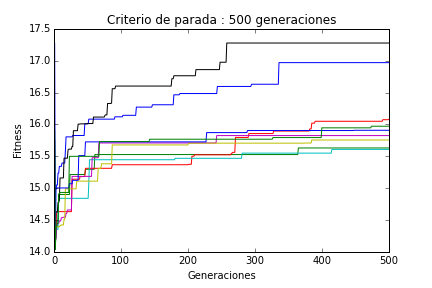
\includegraphics[width=0.8\linewidth]{Figures/criterio_parada}
\caption{Resumen representativo de ejecuciones del algoritmo para establecer el criterio de parada.}
\label{fig:criterio_parada}
\end{figure}



\subsection{Tamaño de la población}

Para la elección de la población se tendrán en cuenta tres elementos: el valor de \emph{fitness} encontrado, el tiempo de ejecución total y la plataforma de ejecución.

La máxima cantidad poblacional a estudiar está determinada por la infraestructura del Cluster Fing, donde la cantidad máxima de procesadores en el mismo nodo es 64. Teniendo en cuenta que la mejor distribución de trabajo es un individuo de la población por procesador, se determina que la máxima cantidad de población será de 64 individuos.

Luego se eligen dos valores mas para completar el análisis, estos son 32 y 48 individuos por población. Se tiene en cuenta que no son lo suficientemente bajos y son valores con los que se obtiene una distribución adecuada de individuos en la infraestructura. Para las pruebas se realizan 10 ejecuciones del algoritmo por cada tipo de tráfico obteniendo el promedio de esos valores.

La tabla \ref{table:parametro_poblacion} muestra los resultados obtenidos; como se aprecia no existen grandes diferencias en la elección de un número poblacional sobre otro. Por tanto se elige como número de población 32, teniendo en cuenta que el tiempo de ejecución secuencial del algoritmo es el menor y que insume menos recursos al ejecutarse. Esto es importante por utilizar el Cluster Fing que es utilizada por otras personas y con recursos limitados.

\begin{table}[h]
	\renewcommand{\arraystretch}{1.2}
	\caption{Comparación de fitness para distintas poblaciones}
	\label{table:parametro_poblacion}
	\centering
	\begin{tabular}{ccrrcp{2cm}}
		\hline
	    \multirow{2}{*}{\textbf{Población}}& & 
		\multicolumn{2}{c}{\textbf{Fitness}} \\
		\cline{3-4}
		& & {mejor} 
		& {promedio} 
		& \textbf{Tiempo ejecución serial (m)} \\
		\hline
		32 & & {17.28} & 16.37$\pm$0.5 & 10184$\pm$526\\
		48 & & {16.19} & 15.84$\pm$0.3 & 6772$\pm$256\\
		64 & & {17.27} & 16.46$\pm$0.6 & 4853$\pm$155\\
		\hline
	\end{tabular}
\end{table}





\subsection{Probabilidad de mutación y cruzamiento}

Para configurar la probabilidad de cruzamiento (pc) se consideraron tres valores candidatos (0.5, 0.8, y 1) y para la probabilidad de mutación (pm) otros tres (0.01,  0.05,  y  0.1). De las nueve combinaciones posibles, se realizaron tres ejecuciones independientes del algoritmo para cada uno de los tres tipos de tráfico (bajo, medio y alto).  
 
 \begin{table}[H]
 	\renewcommand{\arraystretch}{1.2}
 	\caption{Combinaciones de probabilidad de cruzamiento(pc) y de mutación (pm)}
 	\label{table:parametro_mutacion_cruzamiento}
 	\centering
 	\begin{tabular}{p{1cm}p{1cm}p{3.5cm} }
 		\hline
 		$p_C$& 
 		$p_M$ & 
 		Fitness promedio  $\pm$ desviación estándar\\ 
 		\hline
 		0.5 & 0.01  &  16.09$\pm$0.30\\
 		0.5 & 0.05 &  15.60$\pm$0.17\\
 		0.5 & 0.1  &  16.16$\pm$0.42\\
 		0.8 & 0.01  &  16.04$\pm$0.55\\
 		0.8 & 0.05  &  15.85$\pm$0.32\\
 		0.8 & 0.1  &  16.08$\pm$0.34\\
 		1 & 0.01 &  16.08$\pm$0.45\\
 		1 & 0.05 &  15.82$\pm$0.34\\
 		1 & 0.1 &  16.04$\pm$0.25\\
 		\hline
 	\end{tabular}
 \end{table}
 
Analizando la tabla y la gráfica se puede apreciar claramente que para una probabilidad de mutación de 0.05 se obtienen los peores resultados. Otro dato interesante es que no existe gran diferencia en el resto de las combinaciones.

\begin{figure}[H]
	\centering
	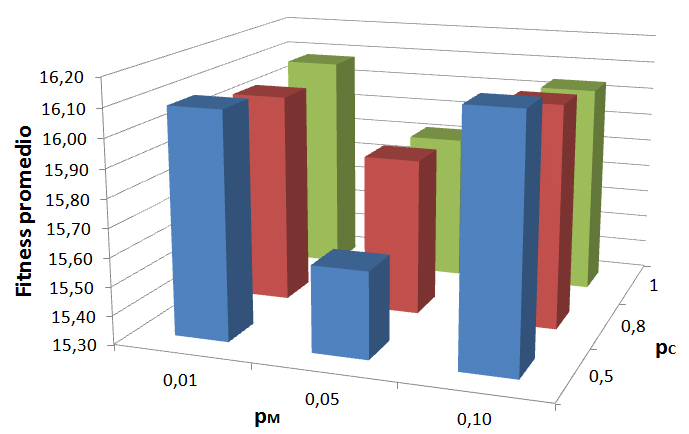
\includegraphics[width=0.8\linewidth]{Figures/grafica_mutacion_cruzamiento}
	\caption{Gráfica con combinaciones de probabilidad de cruzamiento(pc) y de mutación (pm)}
	\label{fig:grafica_mutacion_cruzamiento}
\end{figure}


Se comprueba que todas las muestras siguen la distribución normal para poder aplicar el test de Student. 

%Siendo las hipótesis de la prueba u1 el promedio del  grupo 1 y u2 el del grupo 2)
%
%
%        \begin{equation}
%        \label{eq:student_eq}
%			\begin{split}
%				H0: u1  = u2  \\
%				H1: u1 != u2 
%			\end{split}			
%        \end{equation}

Si se compara la combinación del mejor promedio (0.5-0.1) y del peor (0.5-0.05) con el test de Student obtenemos t(x) = 0.07 que nos indica que para un nivel de significancia de  0,1 la hipótesis nula es rechazada, por lo tanto existe evidencia estadística para elegir la combinación con el mejor promedio (0.5-0.1) sobre la combinación con el peor promedio (0.5-0.05) para la ejecución del algoritmo.

Para comprobar si es la mejor opción  se toman las dos combinaciones con el mejor promedio (0.5-0.1) y (0.5-0.01) obteniendo en el test Student t(x) = 0.71 que nos indica que no existe una diferencia significativa entre ambas muestras por lo que elegir una sobre otra no implicaría grandes beneficios.

En tal sentido podríamos elegir cualquiera de las dos, en este caso se elige  la combinación (0.5-0.01) por su buen promedio y baja desviación estándar.



\section{Descripción de escenarios}
En esta sección se presentan los escenarios que serán evaluados, el primero es el escenario base que representa la realidad actual y el segundo un escenario alternativo que contiene modificaciones con el objetivo de obtener mejores métricas que el escenario base.

\subsection{Caso base o realidad actual del corredor}
El caso base representa la situación actual en términos de tráfico, red vial y sincronización de semáforos del corredor Garzón. El objetivo es realizar una simulación para recabar mas información (velocidad promedio de vehículos y ómnibus) que sirva para comparar con los resultados del algoritmo utilizando los datos obtenidos in-situ (configuración de semáforos, cantidad de vehículos, etc). 

Se valida su correctitud comparando los tiempos obtenidos en la simulación con tiempos obtenidos in-situ de los recorridos de ida y vuelta para los vehículos. Para el caso de los ómnibus se utilizan las frecuencias, cantidad y recorridos de los mismos que son de acceso público.

Se realizó un estudio sobre datos proporcionados por la IMM que contenían el posicionamiento de los ómnibus, velocidad instantánea y datos de la línea durante todo el día para una semana en particular. De esta forma se constató que para las líneas de ómnibus que pasan por Garzón la velocidad promedio de los ómnibus es de 14.5 km/h. Esto permitió calibrar el escenario modificando aspectos de la simulación relacionados con los ómnibus para mayor precisión.

Sobre el escenario base geográfico se realizarán tres escenarios de tráfico : bajo, medio y alto.
El caso medio representa los datos obtenidos en el trabajo de campo, el bajo es disminuyendo el 50\% de vehículos y el tiempo de espera en las paradas de ómnibus teniendo en cuenta que en este caso existirá menos personas utilizando el transporte público. Las frecuencias de ómnibus se mantienen iguales ya que no son alteradas en la realidad.
El caso de tráfico alto se aumenta 50 \%  los vehículos y el tiempo de espera en la parada de los ómnibus. El aumento y disminución del 50\% se obtuvo al analizar datos proporcionados por la IMM de la zona de Garzón de años anteriores. \newline

A continuación el resumen de la cantidad vehicular para los tres escenarios de tráfico:

\begin{itemize}
\item Tráfico Alto:  3000 vehículos en la simulación y 70 ómnibus. 
\item Tráfico Medio: 2000 vehículos y 70 ómnibus.
\item Tráfico Bajo:  1000 vehículos y 70 ómnibus.
\end{itemize}

 

\subsection{Escenario alternativo}

Para mostrar la utilidad que tienen las simulaciones sobre un escenario real, se realiza un escenario alternativo. Una de las ventajas principales es que no requiere gran inversión monetaria, de tiempo y que no afecta la situación actual de la realidad, por lo que se pueden generar distintas pruebas para encontrar aquellas que logren un beneficio.

Analizando los puntos que se entienden podrían atentar contra el buen funcionamiento del Corredor, se agregan algunas modificaciones al escenario base para intentar mejorarlo. 

El objetivo no es demostrar que será la mejor alternativa, sino dar una de las muchas alternativas que se pueden generar y probar con la simulación si se logran mejoras. Ya que pueden existir limitaciones o reglas que no estamos tomando en cuenta y que deben cumplirse en la realidad.

Entre los cambios estudiados se encuentran: eliminación de paradas y pasajes peatonales, alternar paradas y modificación de reglas de semáforos.



\section{Resultados}
En esta sección se muestran los resultados obtenidos tanto de la simulación de la realidad, como de la aplicación del algoritmo. Se presenta la simulación del escenario alternativo y la posterior evaluación. Además se realizan estudios sobre cambios en la función de fitness del algoritmo y un breve análisis de la eficiencia computacional.


\subsection{Valores numéricos del caso base}

En la tabla \ref{table:resultado_caso_base} se pueden ver las métricas obtenidas para las diferentes instancias de tráfico simulado para el caso base. Estos datos representan la realidad actual del Corredor Garzón. Como se aprecia la velocidad promedio de los ómnibus en tráfico medio es de 14.6km/h siendo 14.5km/h el valor que se obtuvo de analizar los datos reales proporcionados por la IMM, lo que verifica que el modelo se aproxima a la realidad. 
 
 \begin{table}[H]
 	\renewcommand{\arraystretch}{1.2}
 	\caption{Resultados del caso base mostrando la velocidad promedio ómnibus (vpb) y velocidad promedio vehículos(vpv) para los distintos tipos de tráfico}
 	\label{table:resultado_caso_base}
 	\centering
 	\begin{tabular}{p{2.5cm}p{2.5cm}p{2.5cm}p{2cm} }
 		\hline
 		&
 		$vbp(km/h)$& 
 		$vvp(km/h)$ & 
 		Fitness \\ 
 		\hline
 		Tráfico Bajo & 15.89  & 32.45& 13.42\\
 		Tráfico Medio & 14.59  & 28.81& 12.05\\
 		Tráfico Alto & 14.31  & 26.36& 11.30\\

 		\hline
 	\end{tabular}
 \end{table}
 
 En el caso base no se representa la desviación standard ya que los resultados de su simulación son constantes, pues siempre se están probando los mismos recorridos de los vehículos y la configuración de los semáforos no cambia. Cuando se aplica el algoritmo obtenemos un valor diferente de velocidad y \emph{fitness} en cada ejecución ya que tienen distintas configuraciones de semáforos, en este caso si se muestra la desviación standard.


\subsection{Resultados numéricos de la evaluación }

Como se aprecia en la tabla \ref{table:resultado_caso_base}, el algoritmo mejora la velocidad promedio tanto de ómnibus como de otros vehículos en los tres tipos de tráfico estudiados. Además la velocidad media de los vehículos se mantiene en un rango mucho más ajustado que en el caso original al variar el tráfico. Las mejoras logradas en el \emph{fitness} son de de hasta 24\%. A continuación se describe el análisis estadístico para comprobar la mejora.


\begin{table}[H]
	\renewcommand{\arraystretch}{1.2}	
		\centering
	\caption{Resultados luego de ejecutado el algoritmo mostrando velocidad promedio ómnibus (vpb) y  de otros vehículos(vpv) para los distintos tipos de tráfico }
	\label{table:resultado_caso_algoritmo}
	\begin{tabular}{cccccccc}
		\hline 
		Tráfico& 
		$vbp(km/h)$& 
		$vpv(km/h)$&
		\multicolumn{2}{c}{\emph{Fitness}}&  & 
		\multicolumn{2}{c}{Mejora \emph{fitness} (\%)}\\  \cline{4-5} \cline{7-8}&     &     & \multicolumn{1}{c}{Promedio} & \multicolumn{1}{c}{Mejor} &  & \multicolumn{1}{c}{Promedio} & \multicolumn{1}{c}{Mejor} \\ \hline
		Bajo & 17.92$\pm$0.18 & 34.30$\pm$0.40 & 14.50$\pm$0.14 & 14.88 & & 8.04 & 10.8  \\
		Medio& 16.95$\pm$0.32 & 33.29$\pm$0.29 & 13.95$\pm$0.15 & 14.19 & & 15.70& 17.7\\ 
		Alto & 16.51$\pm$0.61  & 32.90$\pm$0.25& 13.72$\pm$0.17 & 14.04 & & 21.40& 24.2\\	
		\hline	    
	\end{tabular}
\end{table}

Se realizaron 20 ejecuciones independientes para cada tipo de tráfico comprobando que siguieran una distribución normal.Por tanto se puede aplicar el criterio de significancia estadística para validar los resultados. Este indica que el
algoritmo A es mejor que B si los resultados de A y B cumplen:

\begin{equation}
\label{eq:funcion_significancia}
\left |f_{avg}(A) - f_{avg}(B)  \right | > max(std(f_A),std(f_B))
\end{equation}

En este caso A representa el algoritmo y B el caso base. Esto indica que la diferencia del resultado promedio del algoritmo restado al resultado del caso base debe ser mayor a la máxima desviación. Esto se cumple para todos los casos, por lo que se puede afirmar  que existe evidencia estadística para indicar que los resultados del algoritmo son mejores al del caso base.

\begin{figure}[H]
	\centering
	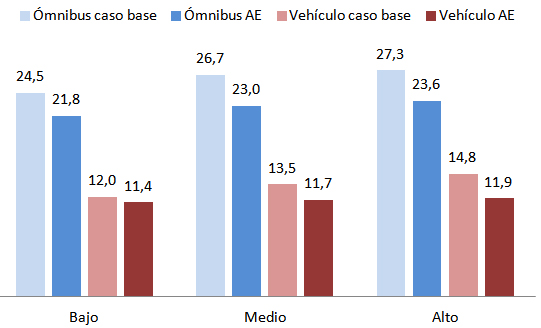
\includegraphics[width=0.8\linewidth]{Figures/duracion_viajes}
	\caption{Comparación de la duración en minutos de los viajes para ómnibus y otros vehículos en el recorrido completo del corredor Garzón para los diferentes tipos de tráfico.}
	\label{fig:duracion_viajes}
\end{figure}

Un resultado interesante es que la duración original de los viajes cuando el tráfico es bajo es casi igual a la duración de los viajes con tráfico alto luego de ejecutar el algoritmo.
Para ómnibus tenemos 24.5m y 23.6m y  para otros vehículos 12.0m y 11.9m.

\subsection{Detalles del escenario alternativo}
Los cambios propuestos incluyen eliminación de paradas, semáforos, pasajes peatonales y alternar paradas. Se estudiaron otras propuestas pero fueron descartadas por la poca viabilidad real de las mismas, como por ejemplo construir calles paralelas a Garzón o nuevas reglas en los cruces como existen en otros países.

\subsubsection{Eliminación de paradas}
Se consideraron dos paradas a eliminar que cumplieran con algunas características: no fueran cercana a una calle principal, que existiera otra parada cercana y que la eliminación de la parada no afecte en demasía a la gente en un traslado mayor.
En este caso se seleccionaron las paradas en la calle Ariel y Casavalle.

\subsubsection{Eliminación de pasajes peatonales}
Hay tres pasajes peatonales en el corredor con semáforos que detienen el tráfico, dos de ellos solo manejan una esquina (sin pulsador en funcionamiento) donde en el escenario alternativo se implementó solamente mediante un \emph{pare} en la calle transversal al corredor y el otro es netamente peatonal frente a la Facultad de Agronomía que fue totalmente eliminado. Una opción que mantiene los pasajes peatonales así como también los resultados obtenidos en el escenario alternativo sería implementar el pasaje peatonal por encima del corredor. Al eliminar los pasajes peatonales se aumenta la velocidad media de todo el transporte.

\subsubsection{Alternar paradas}

Uno de los problemas del ómnibus es su baja aceleración por lo que cada vez que este frena en un semáforo o en una parada demora en retomar una velocidad aceptable. Por tanto al reducir la cantidad de paradas que un ómnibus tiene que hacer se mejora la velocidad promedio.
La línea G recorre a Garzón de punta a punta, es cubierta por las empresas Coectc y Cutcsa. Una posibilidad de alternancia de paradas consiste en dividir las paradas por empresa y compartir las ganancias del corredor u otro método para equiparar el pasaje transportado. 

\begin{figure}[H]
	\centering
	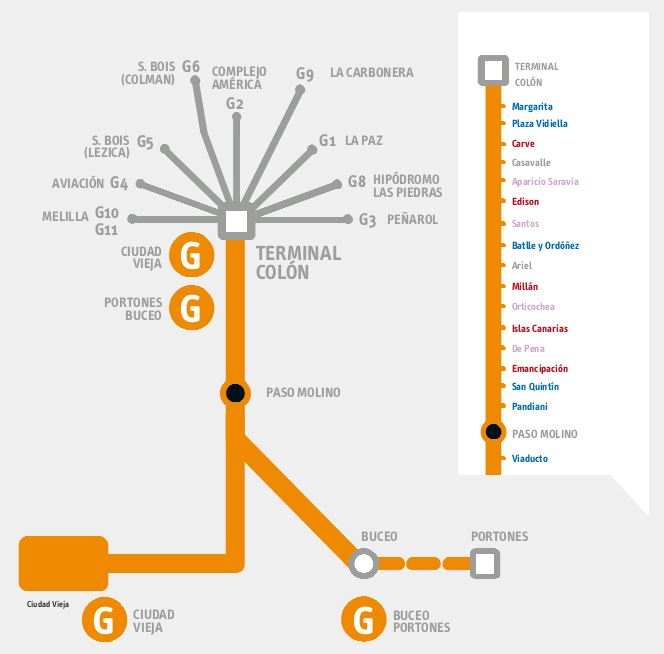
\includegraphics[width=0.9\linewidth]{Figures/paradas_alternativas}
	\caption{Gráfico de paradas alternativas. Gris: Parada Eliminada. Azul: línea G de Coectc y de Cutcsa. Rojo: línea G de Coectc. Violeta: G de Cutcsa. - Imagen original extraída de montevideo.gub.uy}
	\label{fig:paradas_alternadas}
\end{figure}

Una empresa se detendrá en las paradas pares y la otra en las impares y algunas de mayor aglomeración de pasaje/tiempo serán realizadas por las dos. Cada empresa viajará por el corredor a 4 minutos de frecuencia (como en la actualidad). Si se reduce el número de paradas que hace un ómnibus, aumentará su velocidad promedio y no se deberá resentir en demasía el servicio ya que la disminución de la frecuencia en una parada se contrarresta con el aumento promedio de velocidad.

El cambio de alternar paradas es el que más aumenta la velocidad media y tal vez es uno de los más sencillos de implementar en la realidad.



\subsubsection{Cambio básico de semáforos}
Al hacer el relevamiento de los datos se encontró que en todas las intersecciones en donde una línea de ómnibus que circula por el corredor tiene un viraje a la izquierda, se hace detener el tránsito de la derecha de la misma, cada vez que el corredor central tiene la luz verde. Esto no parece tener mucho sentido ya que podrían seguir circulando por el corredor sin ningún tipo de problema, el carril que hay que detener es el de la izquierda del ómnibus cuando una línea dobla a la izquierda pero no los dos carriles al mismo tiempo. No se tiene conocimiento si esto corresponde a un error en la configuración, un tema de costos o facilidad para manejar los dos semáforos de los carriles paralelos juntos. Como esto ocurre en varias intersecciones y en ambos sentidos este cambio mejora la velocidad promedio de los autos que circulan por los dos carriles.

Este cambio se aplicó en las siguientes intersecciones:
\begin{itemize}
	\item Islas Canarias: dobla línea 409 hacia la izquierda, orientado a Colón (Norte).
	\item Camino Ariel: doblan líneas como la  2 y la 148 hacia la izquierda, orientado a Paso Molino (Sur). 
	\item Camino Casavalle: dobla línea 174 hacia la izquierda, orientado a Paso Molino (Sur). 
\end{itemize}

\subsection{Valores numéricos al aplicar los cambios}

Para determinar cuales son los cambios que logran mejores rendimientos se elabora la tabla \ref{table:resultado_alternativo}. Esta se basa en el tráfico medio, ya que solo se quiere realizar una comparación sencilla de las mejoras realizadas. Estos cambios son acumulativos, por lo que se hacen uno después del otro. Se puede apreciar que el que logra una mayor diferencia es la utilización de paradas alternadas.


\begin{table}[H]
	\renewcommand{\arraystretch}{1.2}
	\caption{Valores del escenario alternativo con su velocidad promedio ómnibus (vpb) y velocidad promedio vehículos(vpv) comparando el \emph{fitness} para el tráfico medio }
	\label{table:resultado_alternativo}
	\centering
	\begin{tabular}{p{3.5cm}p{2.5cm}p{2.5cm}p{2cm}p{2cm} }
		\hline
		&
		$vbp(km/h)$& 
		$vvp(km/h)$ & 
		\emph{Fitness} &
		Mejora(\%)
		\\ 
		\hline
		Base & 14.59  & 28.81& 12.05 & -\\
		Eliminar Paradas & 15.44  & 29.03& 12.35 & 2.4\\
		Eliminar Peatonales  & 16.02  & 29.32& 12.59 & 4.4\\
		Paradas alternadas  & 19.17  & 28.88& 13.34 & 10.7\\	
		Cambio reglas  & 18.50  & 29.70& 13.39 & 11.1\\				
		\hline
	\end{tabular}
\end{table}

Una vez que se aplican todos las modificaciones sobre el escenario, se realiza un análisis para los demás tipos de tráfico. Como se ve en la tabla \ref{table:mejoras_trafico_alternativo} se obtienen mejores rendimientos en todos los tipos de tráfico estudiados y el mejor rendimiento se obtiene cuando el tráfico es alto. 

\begin{table}[H]
	\renewcommand{\arraystretch}{1.2}
	\caption{Mejoras obtenidas para las velocidades promedio de los ómnibus(vpb) y de otros vehiculos (vpv) en el escenario alternativo para distintos tipos de tráficos }
	\label{table:mejoras_trafico_alternativo}
	\centering
	\begin{tabular}{p{3.5cm}p{2.5cm}p{2.5cm}p{2cm}p{2cm} }
		\hline
		&
		$vbp(km/h)$& 
		$vvp(km/h)$ & 
		Fitness &
		Mejora \emph{fitness}(\%)
		\\ 
		\hline

		Tráfico Bajo & 20.72  & 33.18 & 14.97 & 11.5\\
		Tráfico Medio & 18.50  & 29.70& 13.39 & 11.1 \\
		Tráfico Alto  & 18.60  & 27.17& 12.7 & 12.6\\		
		\hline
	\end{tabular}
\end{table}

Una vez que tenemos el escenario alternativo se procede a aplicarle el algoritmo cuyo resultado veremos a continuación.


\subsection{Resultados de la evaluación sobre el escenario alternativo}

El escenario alternativo supuso una mejora sustancial en comparación con el caso base (11 \% en el valor de fitness). Se procede a aplicarle el algoritmo para determinar si aún hay posibilidad de mejorar los valores de velocidad y \emph{fitness}.


Los resultados obtenidos en la tabla \ref{table:mejoras_trafico_alternativo_algoritmo}  mejoran claramente el rendimiento del escenario alternativo y por supuesto del caso base en todos los tipos de tráfico. Comparando con la realidad actual se logran mejoras de hasta 37\%. 

Al comparar los resultados obtenidos se aprecia que cuanto más densidad de tráfico, mayor es el porcentaje de mejora. Además un resultado interesante es que las diferencias entre los valores de los distintos tipos de tráfico se redujo.




\begin{table}[h]
	\renewcommand{\arraystretch}{1.2}
	\caption{Mejoras obtenidas al aplicar el algoritmo sobre el escenario alternativo. Comparando las velocidades de ómnibus(vpb), otros vehículos(vpv) y el fitness con cada tipo de tráfico contra el caso base o realidad actual.}
	\label{table:mejoras_trafico_alternativo_algoritmo}
	\centering
	\begin{tabular}{cccccccc}
		\hline 
		Tráfico& 
		$vbp(km/h)$& 
		$vpv(km/h)$&
		\multicolumn{2}{c}{\emph{Fitness}}&  & 
		\multicolumn{2}{c}{Mejora \emph{fitness} (\%)}\\  \cline{4-5} \cline{7-8}&     &     & \multicolumn{1}{c}{Promedio} & \multicolumn{1}{c}{Mejor} &  & \multicolumn{1}{c}{Promedio} & \multicolumn{1}{c}{Mejor} \\ \hline

		Bajo & 23.15$\pm$0.36 & 34.43$\pm$0.33 & 15.99$\pm$0.08 & 16.10 & & 19.1& 19.90 \\
		Medio & 21.83$\pm$0.50  & 33.89$\pm$0.22 & 15.47$\pm$0.09& 15.65 & & 28.3 & 29.87\\
		Alto & 21.46$\pm$0.54  & 33.41$\pm$0.38 & 15.24$\pm$0.19& 15.50 & & 34.8 & 37.10\\	
		\hline		    
	\end{tabular}
\end{table}

En la gráfica \ref{fig:duracion_viajes_alernativo} se puede apreciar la comparación en la duración de los viajes. Se produce una gran reducción en la duración de los viajes de los ómnibus en los tres tipos de tráfico, mientras para el caso de los vehículos la mayor diferencia ocurre cuando el tráfico es alto.

\begin{figure}[H]
	\centering
	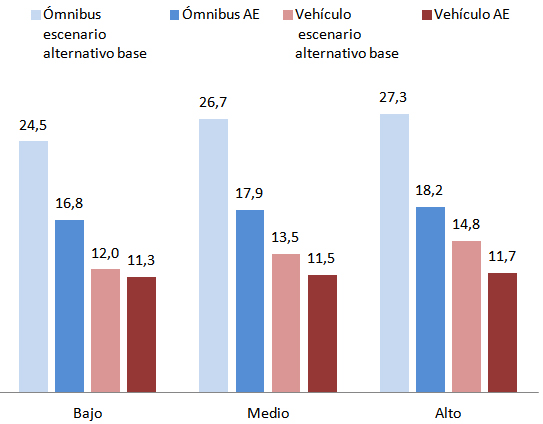
\includegraphics[width=0.8\linewidth]{Figures/duracio_viajes_alternativo}
	\caption{Comparación de la duración en minutos de los viajes para ómnibus y otros vehículos en el recorrido completo del corredor Garzón para los diferentes tipos de tráfico. Al aplicar el algoritmo sobre el escenario alternativo.}
	\label{fig:duracion_viajes_alernativo}
\end{figure}

Otra vez podemos aplicar el criterio de significancia estadística( \ref{eq:funcion_significancia}) para comprobar que la mejora es significativa tanto al comparar con los valores del caso base como con los del alternativo.

\subsection{Variación de la función de \emph{fitness}}

La función \emph{fitness} (\ref{eq:funcion_fitness}) utilizaba los pesos \emph{x = y = 1} lo que representa un balance equitativo  para ómnibus y vehículos.

%Por un cruce de Garzón pasan cada hora:
%70 ómnibus , si aproximamos con 23 personas= 1610 personas por hora
%800 autos, si aproximamos  2 personas por vehículo nos da 1600 personas por hora.
%Una cantidad similar  pasan por el cruce en ambos medios de transporte por lo que no existe una tendencia a favor de una sobre la otra, se podría aproximar que 50\% eligen el ómnibus y 50\% el auto.

Estos pesos pueden ser variados en función de lo que se necesite, por lo que se realizaron pruebas con dos tipos de pesos para comparar como varían las velocidades cuando se da más peso a un tipo de vehículo sobre el otro.


\subsubsection{Prioridad ómnibus}
En este caso se le dará más prioridad a los ómnibus. Esto se sostiene en el hecho que uno de los objetivos buscados por la IMM  es que se utilice más el transporte colectivo como parte de su Plan de Movilidad Urbana \citep{PlanMovilidad}. Con la premisa que al mejorar la duración del viaje en ómnibus en relación al del auto por el corredor, las personas que utilizan auto para sus viajes optarán por el transporte colectivo.

Por tanto se experimentó cambiando los pesos de la función \emph{fitness} con un peso de 70\% para los ómnibus y 30\% al resto de los vehículos.


\subsubsection{Prioridad a otros vehículos}

En este caso, se asignó 70\% del peso a los vehículos y 30\% a los ómnibus. Es el caso opuesto al anterior y resulta útil para poder comparar como varían los valores de las velocidades.

\subsubsection{Resultados}

La siguiente tabla compara las velocidades promedio de ómnibus y vehículos para los tres tipos de pesos que se probaron y por cada tipo de tráfico.  El caso 50-50 es el caso base donde los pesos son iguales, 70-30 es el caso con más prioridad para los ómnibus y el 30-70 más prioridad a los otros vehículos. Se analiza cuanto varían las velocidades de ómnibus (var. vpb) y otros vehículos(var. vpv) comparando contra el caso 50-50 de cada tipo de tráfico.


\begin{table}[H]
	\renewcommand{\arraystretch}{1.2}
	\caption{Modificación de los pesos para ómnibus (pb) y para otros vehículos (pv) en la función \emph{fitness}. Analizando las variaciones en la velocidad promedio de ómnibus (vpb),  otros vehículos (vpv) y \emph{fitness}. }
	\label{table:analisis_fitness}
	\centering
	\begin{tabular}{p{1cm}p{1.2cm}p{1.8cm}p{1.8cm}p{1.8cm}p{1.2cm}p{1.2cm}p{1.2cm} }
		\hline
		Tráfico &
		pb(\%) pv (\%)& 
		vpb & 
		vpv &
		fitness &
		var. \newline vpb(\%) &
		var. \newline vpv(\%) &
		var. \newline \emph{fitnesss}(\%)
		\\ 
		\hline
		& 50-50  & 17.92$\pm$0.18 & 34.30$\pm$0.40 & 14.50$\pm$0.14  &- & - & -\\		
		Bajo & 70-30  & 17.93$\pm$0.23 & 34.06$\pm$0.17 & 12.65$\pm$0.11  & +0.07 & -0.70 & -12.79\\		
		& 30-70 & 17.55$\pm$0.23 & 34.71$\pm$0.21 & 16.42$\pm$0.10  & -2.06 & +1.18 & +13.21\\
		\hline
		
		& 50-50  & 16.95$\pm$0.32 & 33.29$\pm$0.29 & 13.95$\pm$0.15  &- & - & -\\		
		Medio & 70-30  & 17.29$\pm$0.27 & 33.08$\pm$0.14 & 12.24$\pm$0.12  & +2.0 & -0.62 & -12.30\\		
		& 30-70 & 16.71$\pm$0.42 & 33.79$\pm$0.31 & 15.92$\pm$0.11  & -1.41 & +1.49& +14.11\\
		
		\hline
		& 50-50  & 16.51$\pm$0.60 & 32.90$\pm$0.25 & 13.72$\pm$0.17  &- & - & -\\		
		Alto & 70-30  & 16.72$\pm$0.14 & 32.79$\pm$0.26 & 13.75$\pm$0.07  & +1.24 & -0.33 & +0.19\\	
		& 30-70 & 15.48$\pm$0.42 & 33.20$\pm$0.25 & 15.49$\pm$0.16  & -6.23 & +0.92 & +12.87\\
		\hline
	\end{tabular}
\end{table}


Los resultados indican que al variar los pesos de la función \emph{fitness} las velocidades promedio de los vehículos se ve afectada. En el caso de dar más prioridad a los ómnibus se produce como cabía esperar un aumento en su velocidad promedio y una leve baja en la velocidad promedio del resto de los vehículos. Cuando el tráfico es bajo este cambio casi no aumenta la velocidad de los ómnibus. Una explicación posible de este comportamiento es que ya se llegó a un limite máximo y no se puede mejorar más.

Al dar más prioridad a los otros vehículos se produce un aumento en su velocidad y una disminución en la velocidad de los ómnibus la cual es muy evidente en el caso de tráfico alto. Este resultado permite apreciar como estos valores son fuertemente afectados por la densidad de tráfico que se estudie.

En general las variaciones en las velocidades no son grandes pero suficientemente apreciable para tener cierta libertad al plantear distintos objetivos que tiendan a favorecer un tipo u otro de vehículos.


\subsection{Eficiencia computacional}

Se realiza un estudio de la eficiencia computacional del algoritmo para analizar los tiempos de ejecución cuando se usan varios procesadores y como se comporta su capacidad de paralelismo.

Se evalúan nueve ejecuciones del algoritmo; tres con con cada tipo de tráfico: alto, medio y bajo, para estudiarlo en diferentes contextos. El algoritmo utiliza 32 hilos de ejecución por lo que utilizamos esa cantidad de procesadores.

Las pruebas fueron realizadas sobre el node40 del Cluster Fing, con un procesador AMD Opteron 6272 2.09GHz, 48 GB RAM y 32 \emph{cores} utilizados.

El \emph{speedup} (S) mide la mejora de rendimiento de una aplicación al aumentar la cantidad de procesadores comparando con el rendimiento al usar un solo procesador.
\begin{equation}
\label{eq:funcion_speedup}
S = \frac{T_1}{T_N}
\end{equation}
Donde ${T_1}$ es el tiempo de ejecución del algoritmo serial o secuencial, y ${T_N}$ el tiempo del algoritmo ejecutado sobre N procesadores.
\newline

La eficiencia computacional (E) corresponde al valor normalizado del \emph{speedup} (entre 0 y 1) respecto a la cantidad de procesadores. Los valores cercanos a uno indican una alta eficiencia computacional.
\begin{equation}
\label{eq:funcion_eficiencia}
E = \frac{T_1}{N*T_N} = \frac{S}{N}
\end{equation}



\begin{table}[H]
	\renewcommand{\arraystretch}{1.2}
	\caption{Análisis de eficiencia computacional comparando los tiempos de ejecución en serial y paralelo en minutos. }
	\label{table:analisis_speedup}
	\centering
	\begin{tabular}{p{2.5cm}p{2.5cm}p{2.5cm}p{2.5cm}p{2.5cm} }
		\hline
		
		Instancia& 
		Serial(m) & 
		Paralelo(m) &
		\emph{Speedup} &
		Eficiencia
		\\ 
		\hline
		bajo1  & 1572 & 59 & 26.64 & 0.83\\
		bajo2  & 1571 & 59 & 26.62 & 0.83\\
		bajo3  & 1183 & 44 & 26.88 & 0.84\\
		
		medio1  & 3002 & 119 & 25.22 & 0.78\\
		medio2  & 2195 & 82 & 26.76 & 0.83\\
		medio3  & 3007 & 120 & 25.05 & 0.78\\
		
		alto1  & 2920 & 110 & 26.5 & 0.82\\
		alto2  & 4365 & 183 & 23.85 & 0.74\\
		alto3  & 4276 & 177 & 24.15 & 0.75\\
		\hline
		  &  & Promedio & 25.7$\pm$1.1 & 0.80$\pm$0.03\\
		
		\hline
	\end{tabular}
\end{table}


El algoritmo paralelo logra una mejora sustancial en los tiempos de ejecución con un valor promedio del \emph{speedup} de 25.7  y  eficiencia promedio de 0.8, lo cual puede considerarse como buenas métricas.

\begin{figure}[H]
	\centering
	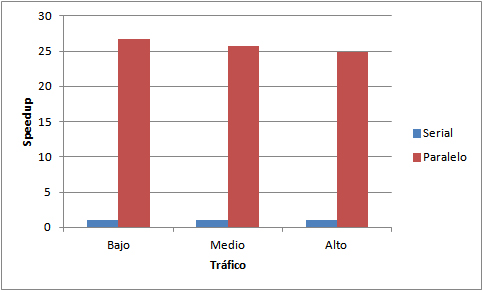
\includegraphics[width=0.8\linewidth]{Figures/speedup1}
	\caption{Comparación de los \emph{speedup} promedios para cada tipo de tráfico. Se representa el caso serial que corresponde al \emph{speedup} = 1 para fines de comparación.}
	\label{fig:speedup1}
\end{figure}

En la gráfica se observa como a medida que aumenta el tráfico disminuye el speedup. Esto sucede por que está influenciado por los accesos al disco duro, al tener más vehículos circulando en la simulación se tiene que leer y escribir más información en los archivos, lo que aumenta el tiempo de ejecución del algoritmo, aunque como se ve no tiene un gran impacto.
\chapter{Conclusiones y trabajo futuro}

\section{Conclusiones}
Al analizar los objetivos planteados al inicio del proyecto, se puede afirmar que las principales metas fueron cumplidas exitosamente.

La investigación de los trabajos relacionados permitió estudiar en profundidad las técnicas de computación evolutiva utilizadas para resolver el problema de sincronización de semáforos, enfocándose en algoritmos evolutivos. En esta etapa, se relevó la información necesaria para formar una base solida en la que se sustenta el diseño de la solución presentada. Se realizó un estudio general sobre la problemática del tráfico, que afecta tanto a la población, como al desarrollo de las ciudades. En la actualidad, se considera imprescindible la búsqueda de soluciones innovadoras y eficientes para mejorar la calidad de servicio ofrecida por las infraestructuras viales urbanas. En nuestro país (Uruguay), no existen antecedentes de propuestas relacionadas con la optimización del trafico urbano. En este contexto, este trabajo plantea un aporte interesante, orientado a estudiar el problema y demostrar que existen las herramientas y el conocimiento necesario para resolverlo.

La sincronización de semáforos es un problema difícil de abordar, en especial al trabajar sobre escenarios reales que revisten complejidad. Sin embargo, las técnicas de inteligencia computacional permiten calcular soluciones eficientes al problema. Se realizaron instancias realistas del problema que modelan la situación actual del Corredor Garzón. Estas instancias contemplan un amplio número de características del problema que proporcionan realismo y aplicación práctica a la solución aportada. El diseño del mapa se basó en información real de la zona, obteniendo el mapa base del servicio OSM. Los datos de tráfico fueron relevados in-situ, siguiendo los lineamientos recomendados en la bibliografía estudiada y de las recomendaciones obtenidas de las reuniones con funcionarios de la división de tránsito de la IMM. Se tuvieron en cuenta las frecuencias reales de las lineas de ómnibus que recorren el Corredor Garzón,  la ubicación correcta de las paradas de ómnibus y las velocidades promedio de los vehículos que fue calculada a partir del análisis de trazas de GPS proporcionadas por la IMM.
 
El enfoque multiobjetivo permitió resolver el problema mediante un enfoque de optimización global, estudiando las velocidades medias de ómnibus y otros vehículos en la zona del Corredor Garzón. El análisis experimental se enfocó en realizar un análisis comparativo con el caso base que representa la realidad actual del Corredor Garzón. Los resultados obtenidos muestran la capacidad de los AE para resolver el problema: el AE propuesto logra una mejora de hasta \textbf{15.3}\% en la velocidad promedio de ómnibus y \textbf{24.8}\% en la velocidad promedio de otros vehículos, obteniendo evidencia estadística que valida las mejoras calculadas.

Se realizaron pruebas experimentales basadas en variar los pesos de la función de \emph{fitness} con el objetivo de dar mas prioridad a un tipo de vehículo sobre otro. Por ejemplo, en el caso de Garzón es interesante estudiar el caso donde se dá más prioridad a los ómnibus sobre el resto de los vehículos, ya que uno de los objetivos del Plan de Movilidad es promover el uso del transporte publico y se considera que al aumentar su velocidad relativa, aumentaría también su uso por parte de la población. Los resultados de estos experimentos mostraron como las velocidades promedio se ven afectadas, aunque las variaciones no son grandes, por ejemplo, al dar mas prioridad a los ómnibus en una instancia de tráfico medio, se logró una mejora en su velocidad promedio del 2\% y una disminución del resto de los vehículos de 0.62\%, comparando con el caso donde las prioridades de ómnibus y otros vehículos son iguales.

Las simulaciones del tráfico demostraron su utilidad al dar la flexibilidad necesaria para probar distintas variantes sobre los escenarios de forma sencilla, y poder diseñar un escenario alternativo realizando modificaciones al escenario base con el objetivo de mejorar las velocidades promedio de los vehículos. Estas modificaciones incluyen: la eliminación de paradas y pasajes peatonales, la modificación de reglas básicas de los semáforos y la alternancia de paradas. La aplicación del AE propuesto sobre el escenario alternativo logra una mejora de hasta \textbf{49.9}\% en la velocidad promedio de ómnibus y \textbf{26,7}\% en la velocidad promedio de otros vehículos comparando con la realidad actual.

El desarrollo de AE con capacidad de paralelización es fundamental, sobre todo en problemas complejos que requieren mucho poder de cómputo, como el abordado en este proyecto. En este trabajo, se implementó un modelo de paralelismo modificando el código base del AE con el objetivo de reducir el tiempo de ejecución, ya que los escenarios evaluados se consideraron complejos y que insumirían mucho tiempo de ejecución. El AE obtuvo buenas métricas de \emph{speedup} lo que permitió reducir considerablemente el tiempo de ejecución del AE al comparar con el caso secuencial. Sin ésta reducción en el tiempo de ejecución del AE hubiera sido muy difícil realizar la cantidad de pruebas presentadas.

\section{Trabajo futuro}
Durante el desarrollo del proyecto, se detectaron varias líneas de trabajo e investigación que seria interesante abordar como trabajo futuro.

El diseño de mapas para la simulación del tráfico requiere la realización de modificaciones para que sean reconocidos por el simulador, en algunos casos se aplicaron manualmente ya que las herramientas no brindaban la granularidad necesaria. Además, la edición de los archivos que representan la configuración de semáforos, las líneas y paradas de ómnibus supone un proceso lento y propenso a errores. Por estos motivos, para un futuro, se sugiere el desarrollo o búsqueda de nuevas herramientas que automaticen o agilicen este trabajo.

El AE desarrollado puede ser aplicado a otros lugares geográficos, modificando  los datos de entrada: mapa, tráfico, configuración de los semáforos y recorrido de ómnibus. El alcance del trabajo sólo se enfocó en la zona del Corredor Garzón, pero sería interesante aplicar el AE en otros escenarios con diferentes características (en el tráfico, en las vías de tránsito, en la cantidad de semáforos, etc) para determinar su capacidad para mejorar las velocidades de los vehículos bajo esas circunstancias.

Un aspecto interesante para desarrollar en el futuro, es el uso de un enfoque multiobjetivo explícito para compararlo con el de agregación lineal utilizado en este proyecto. Para implementar este algoritmo evolutivo multiobjetivo, se podría considerar el uso de otro \emph{framework}, por ejemplo jMetal que incluye varios tipos de algoritmos multiobjetivos.

Los trabajos de  \citet{Montana1996} y \citet{Vogel2000} proponen la adaptabilidad del algoritmo en tiempo real, aunque esto requiere del agregado de sensores a la red, podría resultar en una mejora importante sobre todo, en zonas de gran densidad de tráfico. Se instalarían sensores en los semáforos que detecten la cantidad de automóviles en las intersecciones en tiempo real y un sistema que procesara los datos obtenidos en varias intersecciones para optimizar la circulación del tráfico, modificando la configuración de las luces de los semáforos. El reto de este método se encuentra en que al ser en tiempo real, la configuración de semáforos tiene que ser obtenida relativamente rápida, por lo que el algoritmo utilizado tendría que ser adecuado a esta necesidad.





% -- bibliography --
\addcontentsline{toc}{chapter}{Bibliografía}


%\nocite{*}
{
\bibliographystyle{abbrvnat}
\bibliography{index}	
}

%\renewcommand{\refname}{Referencias}


\end{document}
